\documentclass[12pt]{article}
%\usepackage[showframe]{geometry}% http://ctan.org/pkg/geometry
\usepackage{lipsum}% http://ctan.org/pkg/lipsum
\usepackage{multicol}% http://ctan.org/pkg/multicols
\usepackage{graphicx}% http://ctan.org/pkg/graphicx
\usepackage{float}
\usepackage{fancyhdr}
\usepackage{titling}
\usepackage{subcaption}
\usepackage{indentfirst}
\usepackage{booktabs}
\usepackage{multirow} 
\usepackage{setspace} \doublespacing
\usepackage{mathptmx}
\usepackage{amsmath}
\usepackage[backend=biber, style=apa,]{biblatex}
\usepackage{hyperref}
\usepackage{indentfirst}
\usepackage{float}
\usepackage{caption}

\pagestyle{fancy}
\doublespacing

%\addbibresource{/mnt/c/Users/woute/projects/Thesis_endstop/MyLibrary.bib}
% \addbibresource{/home/wouter/projects/Thesis_endstop/latex_endstop/MyLibrary.bib}
\addbibresource{MyLibrary.bib}

\hyphenpenalty=1000
\tolerance=2000

\fancyhead{}
\fancyfoot{}
\fancyfoot[R]{\thepage}
\renewcommand{\headrulewidth}{0pt}

\setlength{\droptitle}{-10em}   % This is your set screw
\setlength{\parindent}{0pt}

\begin{document}

\captionsetup{font=small}

\begin{titlepage}
\centering

% Adjust font size and family as needed
{\LARGE\bfseries Hierarchical Circuit Structure of Mouse Visual Cortex for Generating Illusory Contour Responses\par}

\vspace{5pt} % Adjust space between title and figure as needed

% Include the figure

\includegraphics[width=0.5\textwidth]{figures/donders_logo.png}

\includegraphics[width=0.5\textwidth]{figures/uva_logo.png}


\vspace{20pt} % Adjust space between figure and author/date as needed

% Author and Date
{\Large Wouter Kroot\par}
\vspace{5pt} % Adjust as needed
{\Large April 2024\par}
\vspace{5pt}
{\Large Supervisor: Prof. dr. P.H.E. Tiesinga}

\end{titlepage}

% Rest of the document starts here
\newpage

% Abstract
\begin{abstract}
  \lipsum[1]
\end{abstract}

\newpage

\section{Introduction}
% a paragraph is around 200 -300 words containing: 

% - Begin with a topic sentence that clearly states the main point or focus of the paragraph. Sets direction and tone informing content and how it relates the the main question or thesis.

% - Necessary background information including definitions a breif review of relevant literature or disucssion of how issue has been approached in the field.

% - Evidence that support point such as data and quantification. substantiates your claims but also shows engagement with tthe existing body of knowledge

% - Analysis of what this evidence means, discuss meaning in the context of my work.

% - Concluding sentence that ties the evidence to the next paragraph. Use: forecasting hinting at the next topic, Linking using literally connecting them with: Furthermore, Additionally, in contrast. 

%------------------------------------------------------------------------------------------------
% Visual image segmentation and illusory contours

\subsection{Recurrent activity is essential for robust image segmentation.}

\setlength{\parindent}{12pt} The mammalian visual system is a complex network of interconnected areas that together process visual information to generate a coherent representation of the external world. An essential part of this process is the ability to segment visual scenes into objects distinct from their background \autocite{kirchbergerEssentialRoleFeedback2020}. Early visual areas, such as the primary visual cortex (V1), perform a local analysis of visual features with relatively small receptive fields and feed their output to higher visual areas (HVAs) that integrate that information over a larger spatial extent and process increasingly abstract features such as object category \autocite{ashbridgeEffectImageOrientation2000}. Visual input in V1 is often clearly defined, e.g., by a luminance contrast that indicates a discontinuity such as an edge or a corner. In other cases, feedforward information is more ambiguous or incomplete and requires further processing for a robust global representation. For example, when an object is occluded by another object, the visual system must make perceptual inferences about the occluded figure and have to fill in the missing details. It has been hypothesised that filling in missing information involves recurrent processing between lower and HVAs \autocite{wyatteEarlyRecurrentFeedback2014}. Recurrent connectivity allows for the integration of local and global visual features and thereby helps the refinement of those representations. Recurrent connections include both horizontal connections within an area and their induced feedback connections \autocite{roelfsemaCORTICALALGORITHMSPERCEPTUAL2006,shushruthStrongRecurrentNetworks2012}. Interestingly, particular stimulus configurations can induce the perception of an occluding figure while no contour is physically present, these are also known as illusory contours. Because these illusory contours are a direct product of the underlying neural circuitry, they can effectively be used to investigate the neurophysiological interactions required to make such visual inferences.
\setlength{\parindent}{0pt}

\subsection{Illusory contour representation in the visual cortex}
Although many configurations are possible to create illusory contours, they often share common features \autocite{palmerLateInfluencesPerceptual2000}. Consider the abutting grating illusion \autocite{sorianoAbuttingGratingIllusion1996} and the Kanizsa triangle illusion \autocite{kanizsaSubjectiveContours1976}. Both illusions involve extrapolations from visual cues that suggest the presence of an occluding object. In the abutting grating illusion, the misalignment of lines creates the impression of a vertical contour superimposed on horizontal inducers \hyperref[fig:figure_1]{(figure 1 a.)}. Similarly, in the Kanizsa triangle illusion, three pacman-shaped figures are arranged such that a continuous contour seems to connect the edges of these inducers \hyperref[fig:figure_1]{(figure 1 b.)}. Although both figures consist of seemingly simple geometrical forms, for the resulting figure to emerge from the background inducers, they require sophisticated processing of individual inducer shapes, their relative position and orientation. This inter-object complexity necessitates the integration of segmented stimuli, possibly involving feedback or recurrent activity. Single-unit recordings from cats and primates have identified particular neurons in the early visual cortex that react to subjective contours similar to how they respond to real lines \autocite{leeDynamicsSubjectiveContour2001,vonderheydtMechanismsContourPerception1989}. Notably, the response times in the secondary visual area (V2) precede those in V1. Indicating that the first place sensitivity to illusory contours arises in the rhesus macaque is V2. Recurrent processing has been demonstrated to be an important part of perceptual organisation \autocite{roelfsemaCORTICALALGORITHMSPERCEPTUAL2006}. In that recurrent processing can support grouping of behaviourally relevant objects and separates objects from the background. This recirculation of information is associated with synaptic and conduction delays and would fit the times delays observed during the filling in process of illusory contours (55 ms) \autocite{leeDynamicsSubjectiveContour2001,pakTopDownFeedbackControls2020}. If V2 illusory responses are due to recurrent activity and real and illusory contours are processed by the same cells, a direct implication would be that higher visual areas might be unable to distinguish between real and illusory contours.

\begin{figure}[H]
    \centering
    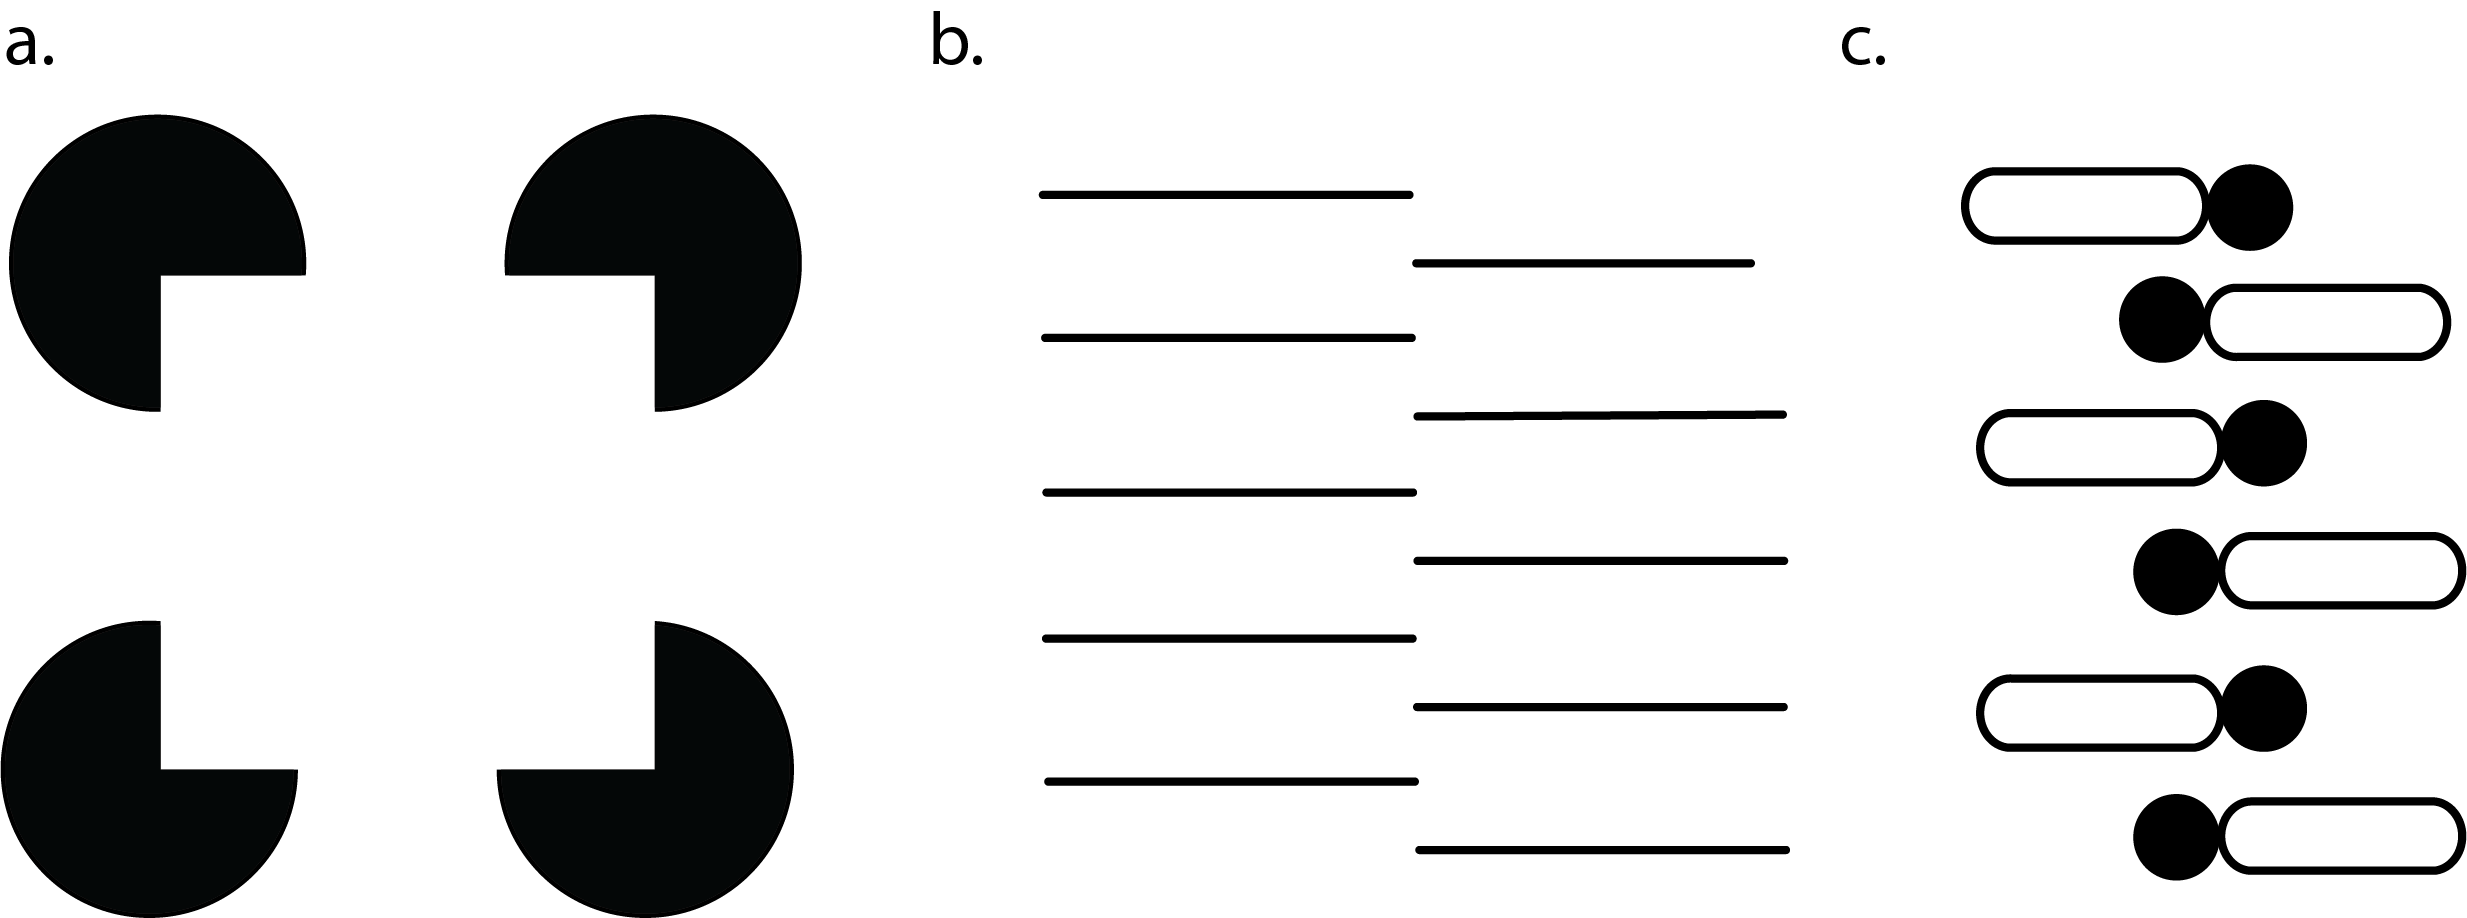
\includegraphics[width=1.0\textwidth]{adjusted_figures/illusory_figure.png}
    \caption{a. The kanizsa illusion \autocite{kanizsaSubjectiveContours1976}. Four pac-man shaped inducers can be perceived as four circles with an overlapping white square. b. The activity elicited in mouse V1 by the Kanizsa triangle. After mapping the receptive fields of a set of neurons the Kanizsa inducers were placed such that the receptive fields of these neurons were not stimulated by feedforward input. Still, the neurons responses were measured due to feedback signals related to the illusory contour.
    c. The Abutting grating illusion \autocite{sorianoAbuttingGratingIllusion1996}. The alignment between the horizontal inducers gives the impression of a vertical contour. d. The proposed neural mechanism for the detection of these visual features are endstopped cells, which can be characterised by an elongated receptive field with an inhibitory endzone.}
    \label{fig:figure_1}
\end{figure}



%ToDo talk about the figure and check whther the references are good
\subsection{Illusory contours are controlled by top-down projections.}
This hypothesis has been examined, with area V4 in the macaque identified as a crucial integration point where both real and illusory contours are represented equivalently \autocite{panEquivalentRepresentationReal2012}. Through the use of optical imaging and single-cell recordings to compare neural activity elicited by real and illusory contours across areas V1, V2, and V4, it was found that activities in V1 and V2 predominantly relate to the encoding of local spatial features of the inducers, rather than the global orientation of the illusory contour. Meanwhile, V4 processed both real and illusory contours similarly, indicating that hierarchical interactions might govern the global orientation processing of illusory contours. This suggests that feedback mechanisms could account for the selective stimulation and orientation tuning of V2 cells in response to illusory contours. Additional support for the vital role of feedback in the representation of illusory contours is provided by studies illustrating the interactions between V1 and the lateromedial visual area (LM) in mice during the perception of illusory contours \autocite{pakTopDownFeedbackControls2020}. These studies trained mice to differentiate between stimuli with and without illusory contours, linking their behaviour to neural activity. Given the extensive genetic toolkit available for mice that allow for the precise recording and stimulation of specific cells, they are exceptionally well-suited for investigating the hierarchical processing that underpins perceptual inferences. The findings revealed that, akin to macaques, mice also exhibited a delay (30 ms) in the representation of illusory contours compared to those defined by contrast, suggesting that the processing of illusory contours involves a more complex integration of visual information than that of contours directly derivable from sensory input. Moreover, the representation of illusory contours in V1 was eliminated upon silencing of LM through optogenetics, indicating a possible similarity in the processing relationship between V1 and LM in mice and that between V2 and V4 in macaques, which aligns with theories of recurrent processing \autocite{wyatteEarlyRecurrentFeedback2014}. Additionally, recent research \cite{shinRecurrentPatternCompletion2023} found that a specific subset of V1 cells in mice could complete the perception of an illusory contour when sufficiently stimulated. Employing decoding techniques and 2-photon stimulation, it was demonstrated that activating a particular small set of V1 cells (5\%) could suffice to generate the perception of illusory contours across the V1 network, without any visual stimulation. These findings propose a model where  recurrent feedback activity in V1 underlies illusory contour representations, highlighting the necessity for further investigation into how these cells are precisely targeted based on the configuration of inducing stimuli.

%ToDo: add papers by Shin for the L2/3 IC cells (Will be a population in the grand model)
  %Write out the importance of Layer 2/3 as the integration point of feedforward and feedback

% Compare monkey and mouse visual areas, strategy image segmentation {luongo 2023}
\subsection{Hierarchical structure of Mouse and Macaque Visual Systems.}
Due to their ability to perceive illusory contours and the relative simplicity of their visual pathways compared to primates, mice offer a unique opportunity for studying both local and hierarchical processing during image segmentation. Whilst the mouse visual cortex comprises roughly nine areas \autocite{wangAreaMapMouse2007}, the primate visual cortex extends across approximately 30 areas, accounting for over half of their neocortex \autocite{fellemanDistributedHierarchicalProcessing1991}. This anatomical disparity is reflected by the fact that mice do not primarily rely on their vision and that they are limited in their ability to segment figures from ground compared to primates \autocite{luongoMicePrimatesUse2023}. Nevertheless, mice have demonstrated the ability to utilise texture-based strategies for figure-ground discrimination, in which patterns with different orientation and or phase are used \autocite{kirchbergerEssentialRoleFeedback2020}. Understanding how illusory contours are represented in the mouse visual cortex using computationally straightforward methods could offer insights that are generalisable to the more complex integrations observed in the primate visual cortex. Interestingly, both the mouse lateral medial area (LM) and the primate V2, which are implicated in the generation of illusory contours, represent the vertical meridian along their borders with V1, suggesting that LM could be the homologue of primate V2 \autocite{gamanutAnatomicalFunctionalConnectomes2022}. The consistency between illusory contour representation highlights the potential to generalise findings from mice to primates. Furthermore, primates and mice also share visual processing functions, such as orientation and spatial frequency selectivity \autocite{niellHighlySelectiveReceptive2008}. This similarity indicates that is might be possible that primates process illusory contours based on these basic visual features. Therefore, it is important to mechanically explain the representation of illusory contours in a simplified setting with a computationally straightforward method using visual features like orientation selectivity and retinotopic integration. Importantly, processing information within the cortical column follows a hierarchical structure, in mice as in primates. There is a clear distinction between feedforward and feedback connections. In primates, feedforward projections arise mostly from supragranular layer 3 as well as granular layer 5, whereas feedback projections originate mainly from infraganular layer 6 and L2/3 \autocite{markovAnatomyHierarchyFeedforward2014}. The feedforward connections mainly target L4, whereas feedback connections tends to avoid L4 \autocite{rocklandWhatWeKnow2019}. The connectivity patterns the cortical column of the mouse is similar to that of the primate, with the main difference being that feedforward connections are not isolated to L4 but also target supra- and infragranular layers. Thus, apart from the small size and relatively lower complexity, mice still have a hierarchical structure similar to that of the primate. Therefore, regarding the generation of illusory contours it is necessary to first examine how orientation selectivity is generated and can be used to recurrently complete a boundary between inducer points.

\begin{figure}[H]
  \centering
  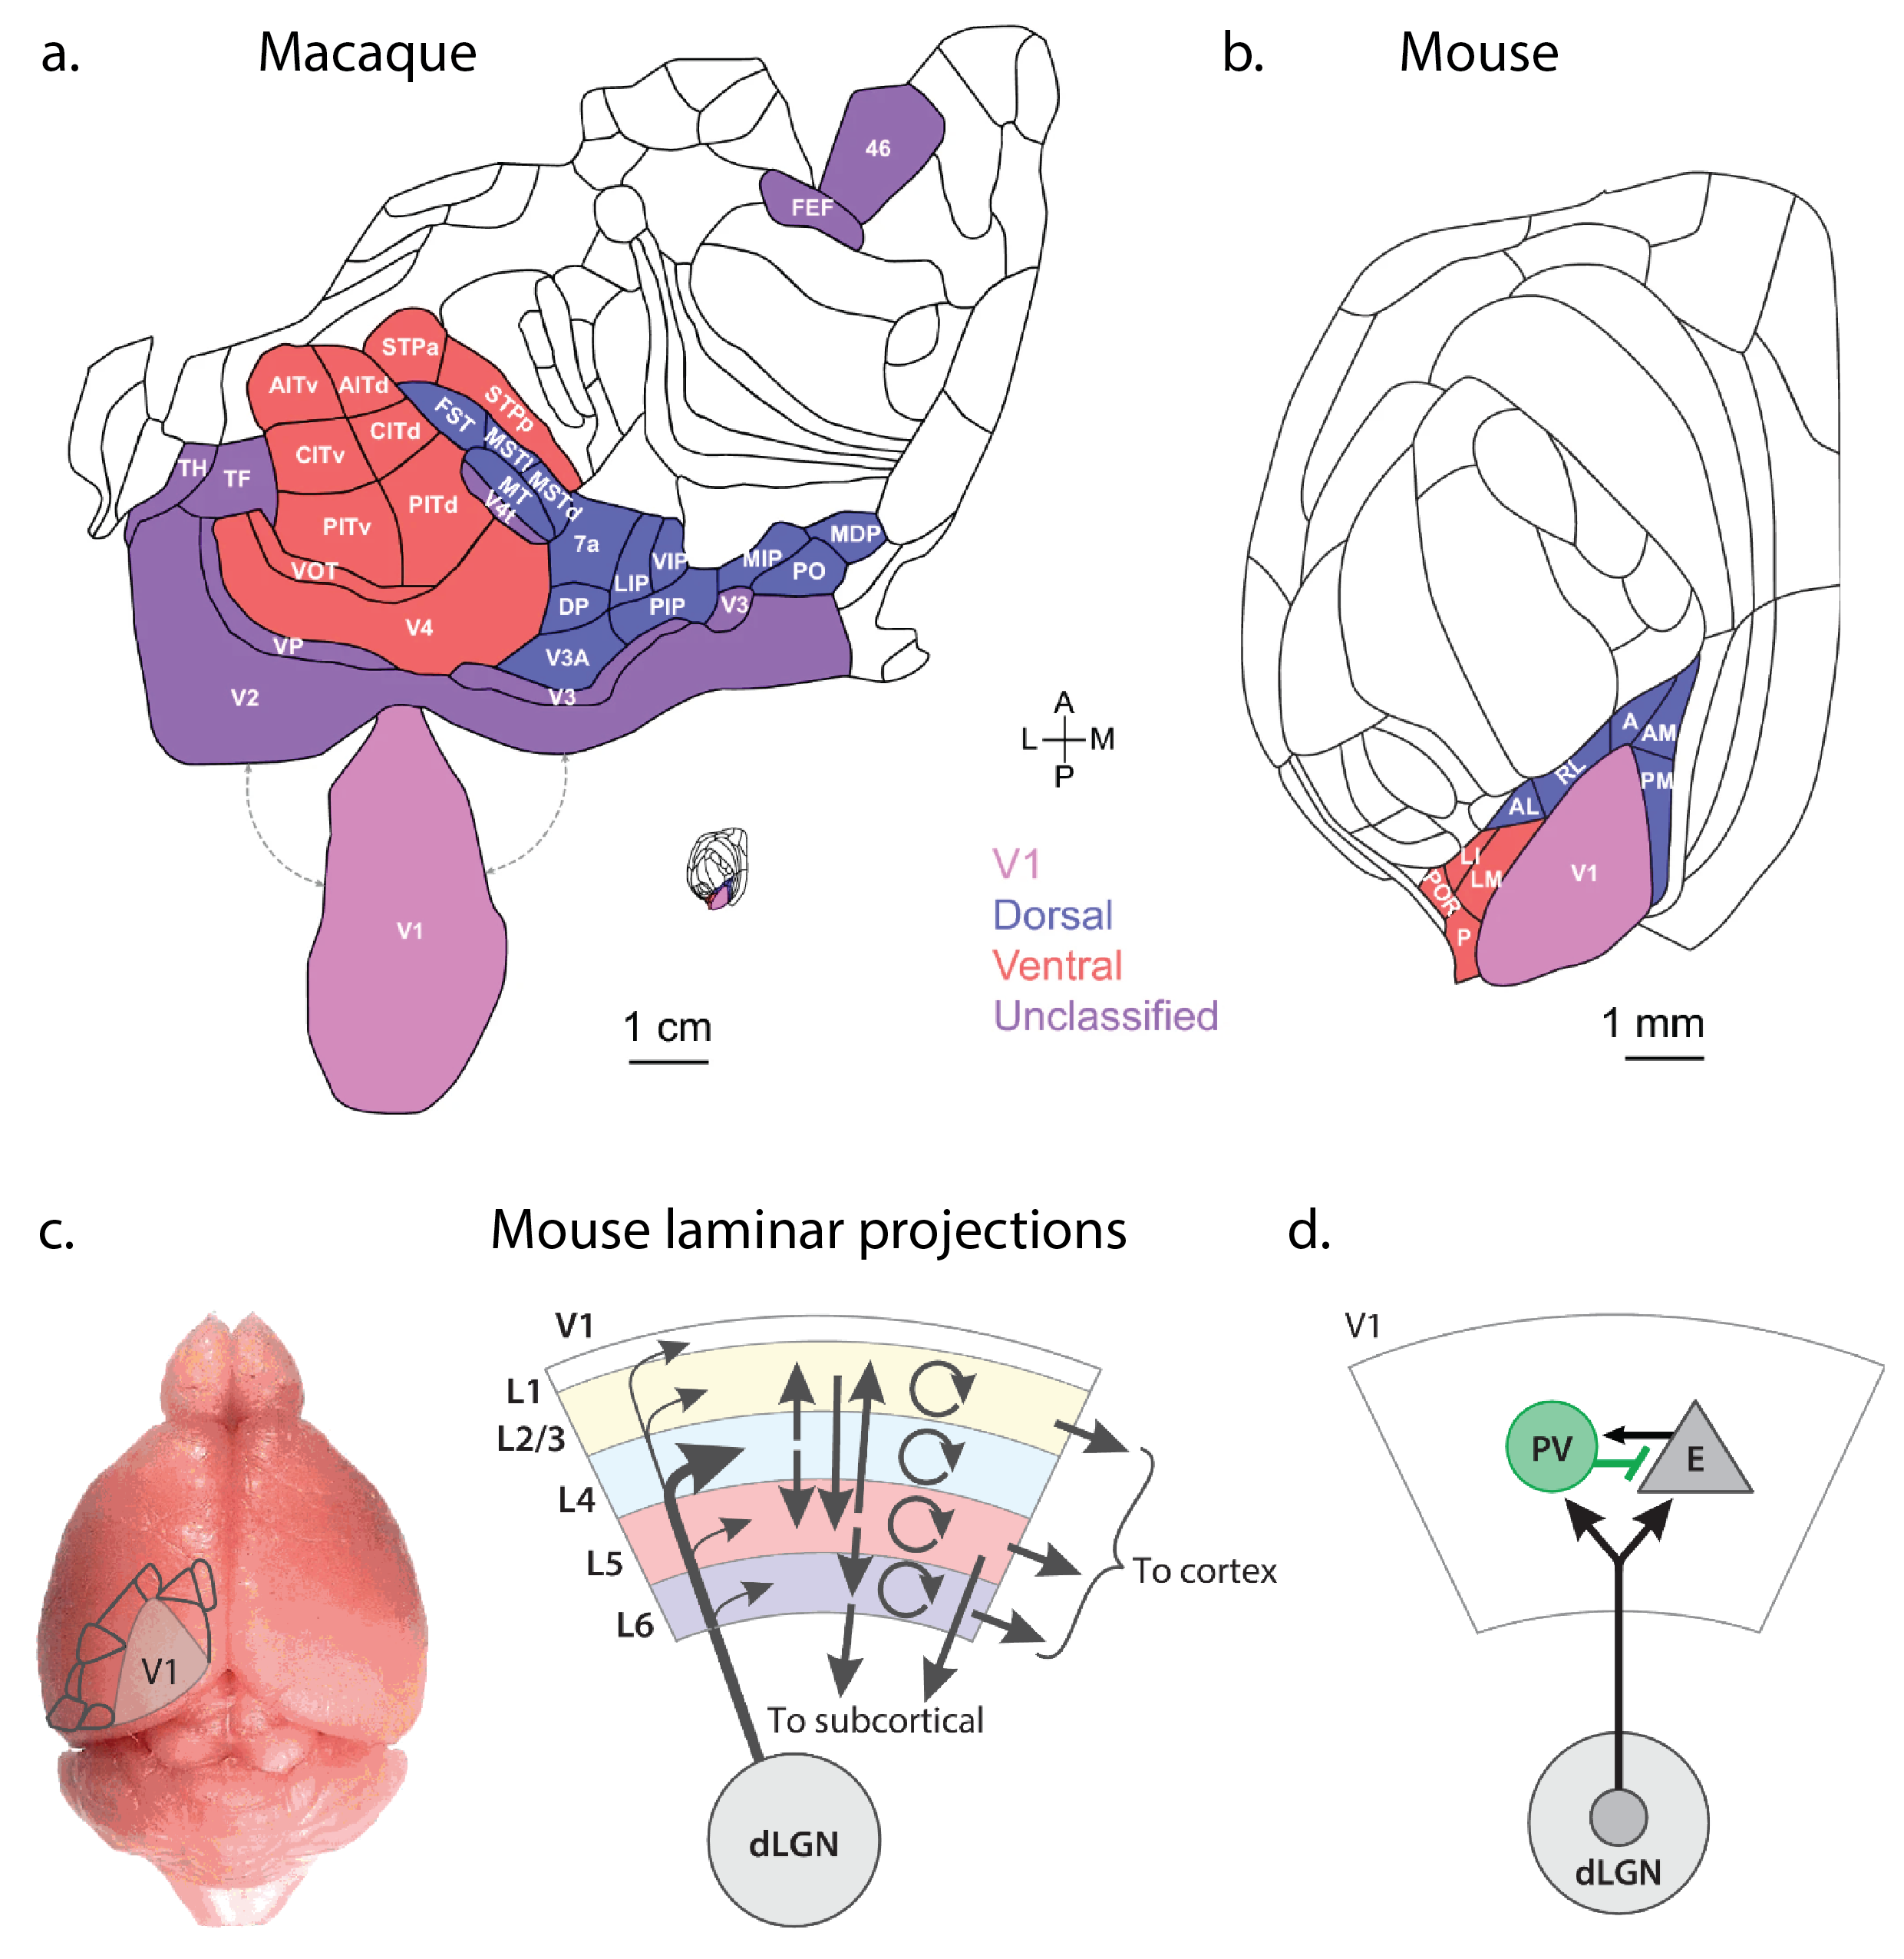
\includegraphics[width=1.0 \textwidth]{adjusted_figures/Laminar_Figure.png}
  \caption{a. The visual system of the macaque, visualising the hierarchical difference with the mouse visual system \autocite{gamanutAnatomicalFunctionalConnectomes2022}. b. The mouse visual system, highlighting the dorsal and the ventral stream, specifically ventral area LM as a potential homologue for macaque V2. c. The visual system mapped on a cortical image and a description of the laminar projections within V1. Similar to the organisation in the macaque, input from the dLGN is predominantly projected to layer 4, which projects to L2/3 and L5. d. Feedforward input mainly targets excitatory pyramidal cells and PV inhibitory interneurons, indicating that these cells might be of importance for the integration of feedforward and feedback signals.
  \autocite{niellHowCorticalCircuits2021}}
  \label{fig:Laminar_Figure}
\end{figure}


% Simple models orientation selectivity and  models for recurrent boundary completion (Grossberg), and deep learning models?

% Orientation selectivity is different in mouse vs primate so talk about models
%- models:
% Hubel DH, Wiesel TN (1962) Receptive fields, binocular interaction and functional architecture in the cat’s visual cortex. J Physiol 160:106–154. Medline
% Nguyen, Freeman 2019, model Hebbian strengthening spatially offset.
% Priebe 2016, Annual review Mechanisms of Orientation selectivity in V1

% - physiology
% Scholl, Corey, Priebe 2013, emergence orientation selectivity mammalian visual pathway
% Niell and Stryker 2008, ighly selective receptive fields in mouse visual cortex 
%- filling in 
% Filling-In the Forms: Surface and Boundary Interactions in Visual cortex
% Mechanism of surface completion: Perceptual Filling-In of texture Spillman De Weerd
\subsection{Orientation selectivity in the visual system.}
To accurately represent an illusory contour, the visual system must be sensitive to the local orientation of the horizontal inducer lines to effectively determine the global spatial relationship between them. V1 is the first visual area where cells sensitive for orientation are found. Both retinal ganglion cells and their target LGN relay cells have circularly symmetric receptive fields and respond to nearly any stimulus within these fields. V1 neurons, however, are responsive to a number of stimulus attributes, such as orientation, motion direction, size, and binocular disparity of visual contours \autocite{hubelReceptiveFieldsBinocular1962}. 
Early models proposed by \textcite{hubelReceptiveFieldsBinocular1962} emphasised the convergence of signals from the dLGN to V1, suggesting a hierarchical integration of visual information. Physiologically V1 neurons can be described as simple or complex cells and are both orientation selective \autocite{skottunClassifyingSimpleComplex1991}. Simple cells receive direct input from the dLGN relay cells and their receptive field responses are characterised by segregated ON and OFF fields that prefer light or dark input, respectively. These subfields are elongated taking on an elliptical shape along the axis of the neuron's preferred orientation \hyperref[fig:LIF_Overview]{(figure 4 a.)}. Due to the segregated ON and OFF subfields their responses are sensitive to changes in phase and polarity \autocite{mechlerClassificationSimpleComplex2002}. 

In contrast, complex cells that receive input from V1 simple cells have receptive fields in which ON and OFF regions are not spatially segregated. Therefore, complex cells respond to both increases and decreases in luminance at the same location and are not sensitive to stimulus polarity or tuned to a particular phase. An important question is how the spatial offset of ON and OFF subfields are developed, since these pathways are not segregated within the LGN. \textcite{nguyenModelOriginDevelopment2019} demonstrated that through a process of Hebbian learning the ON and OFF inputs could be sufficiently segregated to produce orientation selective neurons. In their simulations they simulated a 6 x 6 degree patch of visual field and divide that patch with random ON and OFF channels. Then they stimulated neuronal responses using a drifting grating over the full range of orientations. Each cycle in the development process then consisted of increasing the weights of all synapses for one randomly chosen subcortical channel. If the firing rate of a cortical neuron increased as a result, the synapse between the channel and the cortical target remained strengthened, and was otherwise decreased. After roughly 16000 cycles they found segregated ON and OFF subfields that was sufficient for orientation tuning. Still, the question remains whether a strict feedforward process is also sufficient for orientation tuning in physiology.

To test whether orientation selectivity is a strict thalamocortical feedforward process or that these functional properties are a product of neuronal mechanisms on the cortical level \textcite{fersterOrientationSelectivityThalamic1996} inhibited cortical spiking and measured sub-threshold responses. They found that V1 neuron orientation selectivity is largely unaffected by cortical inactivation, providing evidence that the feedforward information transmitted by the LGN relay cells are sufficient to be transformed into orientation selective responses and that cortical circuitry is not required to refine these responses. Despite evidence showing similarities between mammals for how orientation selectivity originates, there are also large differences in the functional organisation across species. For instance, neurons in mouse V1 are not organised in columns with similar orientation preferences, as in primates. Mice also do not have the same pattern of functional segregation by layer that primates exhibit in which simple cells are found more in L4 and complex cells in deeper L2/3 \autocite{martinezReceptiveFieldStructure2005}. Instead, in the mouse, simple and complex cells are evenly distributed across cortical layers \autocite{niellHighlySelectiveReceptive2008}. Nevertheless, these differences in functional organisation are demonstrated to have a minimal impact on the functional properties of orientation tuning \autocite{hooserOrientationSelectivityOrientation2005}. Understanding the neuronal mechanisms of orientation selectivity across species is fundamental to the goal of understanding more complex perceptual phenomena, such as the perception of illusory contours. This leads us into an examination of various models that attempt to explain how the visual system integrates local and global information to have a shape or contour emerge from inducer shapes.    

\subsection{Models for illusory contour perception}
% Challenging deep learning models with abutting grating. Need for recurrency.

% A widespread view is that most texture segregation can be accounted for by differences in the spatial frequency content of texture regions, simple cells. Evidence from both psychophysical and physiological studies indicate, however, that beyond these early filtering stages, there are stages of 3-D boundary segmentation and surface representation that are used to segregate textures. \autocite{grossbergTextureSegregationSurface1998} (endstopped cells?)
% They arrive at a
% mutually consistent representation through reciprocal
% interactions. These interactions have been interpreted in
% terms of pathways joining the interblob and blob cortical streams between cortical areas V1 and V4 [19]. They
% are here used to explain texture segregation data for
% which early filtering mechanisms are insufficient. (Reciprocal, recurrency)
% endstopped cells for local detection
% bipole AND gate, however are orthogonally tuned, should not be local then larger receptive field HVAs
% biep.

A recent study by \textcite{fanChallengingDeepLearning2023} explores the challenges deep neural networks (DNNs) face in representing illusory contours, specifically through the abutting grating illusion. Illusory contours, such as those seen in theabutting grating illusion, evoke perceptions of boundaries where none exist, a phenomenon that standard edge detectors cannot handle. The study highlights the failure of convolutional neural networks (CNNs) in revealing activity along these contours and proposes that recurrent processing, akin to that in biological vision, is crucial for accurate representation. In biological systems, recurrent connections allow for the integration of contextual information, essential for resolving ambiguities and ensuring consistent perceptual grouping and boundary completion. DNNs, which lack such recurrency, often fail in tasks involving illusory contours, underscoring a significant gap between artificial and biological vision systems \autocite{fanChallengingDeepLearning2023}.

Grossberg, Mingolla, Peterhans, and von der Heydt have significantly contributed to understanding the neural mechanisms behind boundary completion and figure-ground separation. Their models incorporate endstopping and bipole cells to simulate how the brain perceives continuous boundaries from fragmented visual information. Grossberg and Mingolla's neural dynamics model, for instance, explains how visual inputs activate the Boundary Contour System (BCS), which interacts with the Feature Contour System (FCS) through feedback loops to complete boundaries and surfaces. This interaction is critical for the perception of illusory contours and shapes \autocite{grossbergTextureSegregationSurface1998}. Peterhans and von der Heydt expanded on these ideas by demonstrating that endstopped cells in the visual cortex, particularly in V1 and V2 areas, respond to lines and edges, contributing to the perception of illusory contours through mechanisms that integrate local orientation signals into coherent shapes\autocite{grossbergTextureSegregationSurface1998}. These endstopped neurons are maximally activated when lines or edges terminate within their receptive field but deactivate when the lines extend through it, making them crucial for detecting terminations and corners, fundamental elements in creating the perception of contours. Grossberg highlights the need for another cell type, the bipole cell. Bipole cells are senstive to collinear alignment of edges in local boundary detection, they are capable of integrating endstopped cells and can be used to complete open boundaries. Higher visual areas such as V2 and V4 are necessary for integrating information over larger spatial extents and bridging gaps between endstopped points. These areas use feedback connections to complex cells in earlier visual areas, reinforcing and refining the initial boundary signals to create stable and coherent perceptions of illusory contours.

In conclusion, while bipole cells and endstopped neurons play crucial roles in local boundary detection, the full representation of illusory contours requires a more integrated approach involving higher visual areas and recurrent processing. This hierarchical and recursive processing framework enables the visual system to perceive complex shapes and contours that are not explicitly present in the visual input, a sophistication that current DNNs lack. Thus, integrating recurrent connections and feedback mechanisms in artificial vision systems is essential for advancing their capability to mimic primate and mice cortical architectures \autocite{grossbergHowVisualIllusions2014,grossbergTextureSegregationSurface1998}. 

\subsection{Current study local circuit structure for recurrent filling in.}
The abutting grating and Kanizsa illusions are both characterised by congruent illusory inducing points, identifiable by the presence of aligned line endings. Kanizsa inducers are considered more complex than abutting line inducers because each inducer point forms part of a corner, essentially two line ends meeting at an angle. In contrast, the abutting grating illusion is simpler, with its inducer points as single-line ends and, therefore, could be represented by a single endstopped cell \hyperref[fig:figure_1]{(figure 1)}.
Nonetheless, cells sensitive to length might be fundamental to encoding both illusions, known as endstopped cells. Initially classified by Hubel and Wiesel in the cat's primary visual cortex (V1) in 1969, these cells are orientation-tuned and exhibit inhibition when a line segment exceeds their excitatory receptive field, leading to their initial characterization as hypercomplex cells for their complex cell properties, such as stimulus polarity invariance, combined with inhibitory end zones \autocite{hubelRECEPTIVEFIELDSFUNCTIONAL1965}. Subsequent research revealed that a significant portion of V1 neurons exhibit endstopping to varying degrees  \autocite{deangelisLengthWidthTuning1994,jonesSurroundSuppressionPrimate2001,sceniakVisualSpatialCharacterization2001} across different species, including primates, cats, and mice. Computational models have shown that endstopping can sufficiently delineate figures from the background and reconstruct illusory contours \autocite{vonderheydtMechanismsContourPerception1989}, suggesting that endstopped cell integration might serve as a universal neural mechanism for segmenting the visual field and to generating illusory contours.

%ToDo add a section of how endstopping is not caused by direct inhibitory endzones: \autocite{sillitoContributionExcitatoryInhibitory1977}
% Part under here is wrongly cited, has to be worked out again:

Despite these insights, neurophysiological studies have largely overlooked how endstopping is integrated into higher visual areas for illusory contour perception. Previous computational simulations, while informative, have relied on feed-forward convolutions without accounting for biological constraints, such as direct inhibition to simulate negative end zones (Sillito \& Versiani, 1977), and have not incorporated feedback mechanisms now recognised as crucial for the representation of illusory contours in lower visual areas. Addressing this gap, our current research endeavours to simulate endstopping using Leaky Integrate and Fire (LIF) neurons and to integrate endstopped microcircuits through population rate models to accurately represent the abutting grating illusion. Our findings shed light on the minimal microcircuit necessary to exhibit end-stop characteristics, further illuminating how the representation of illusory contours through recurrent activity is modulated by the orientation selectivity of endstopped cells in higher visual areas. By incorporating endstopped cells into a hierarchical model, we aim to elucidate the neural mechanisms underlying illusory contour perception and to provide a comprehensive understanding of how the visual system processes illusory contours.

This study investigates whether endstopping in V1 can occur solely through feedforward signals without direct inhibition or if a feedback mechanism is essential for activating inhibitory end zones. By simulating the representation of the abutting grating illusion via endstopped cell-driven recurrent activity, we explore the physiological constraints on integrating orientation-tuned endstopped cells in higher visual areas. Our goal is to elucidate how endstopped cells contribute to the perception of illusory contours and their integration within the visual cortex hierarchy. We hypothesize that endstopped cells are crucial for the representation of illusory contours and that their orientation tuning is modulated by feedback signals from higher visual areas. Our results will provide insights into the neural mechanisms underlying illusory contour perception and the hierarchical processing of visual information in the mammalian visual system.


\newpage
\section{Methods}
% Introduction that states that we used two models with a rationalisation of why
\noindent \textbf{Spiking neuron and population Model design.} \newline
To investigate the local circuit necessary for endstopping and how endstopping features can be used to generate illusory contours within the visual cortex of the mouse, the current study used two distinct computational frameworks. In the initial phase of the investigation, we utilised leaky integrate-and-fire (LIF) models to simulate the spatial and temporal integration of synaptic input, on the single-cell level. This approach provided a foundational understanding of the mechanisms underpinning orientation selectivity, complex cell features such as polarity invariance, and endstopping. However, the current connectivity between LIF cells was set by hand, and the complexity and computational demands associated with the tuning of each neuron constrained the current study to shift towards population models for the subsequent phase of generating illusory contours. Nevertheless, the LIF network allowed an estimate of the necessary amount of cells needed to create a stable neural mechanism for endstopping, and the population models could abstract this behaviour into a computationally tractable form, enabling the simulation of illusory contour generation efficiently. 

\bigbreak
\subsection{Simulating the Local Circuit for Endstopping using the BMTK.}

To stimulate endstopping behaviour the Brain Modeling Toolkit was utilised to define and connect nodes. To construct an architecture of spiking point neurons it is necessary to initilialise an instance of the NetworkBuilder class provided by the BMTK. The current example will create a network for the dLGN and a network for V1. To present the visual stimuli and connect nodes from the LGN to V1, the Brain Modelling Toolkit was used. This simulation pipeline processed visual information through a series of steps with increasing complexity, starting with presenting the visual stimulus. Visual stimuli were dynamically presented through a three-dimensional array format (t, y, x). Each entry along the first dimension time (t) is a frame with input organised along the vertical (y) and horizontal (x) dimensions. By following these steps, you can effectively use the Brain Modeling Toolkit to create complex neural networks. The toolkit's flexibility allows for precise control over the spatial arrangement and connectivity of neurons, facilitating the modeling of intricate neural circuits and their dynamic behaviors. This guide demonstrates the process of defining, connecting, visualizing, and saving neural networks using BMTK, providing a robust framework for neural network modeling and simulation. An important aspect of BMTK is its support for different simulation environments. In this context, we used two distinct types of simulations: filternet and pointnet. Filternet is employed to simulate the LGN, focusing on the filtering properties of LGN neurons and their responses to visual stimuli. This separate simulation environment is particularly suited for capturing the dynamics of large-scale LGN networks and their pre-processing role in the visual pathway. The importance of using filternet lies in its ability to model the initial stages of visual processing, where the LGN acts as a relay station, refining and filtering visual information before it reaches the cortex. This simulation environment allows for detailed analysis of how LGN neurons process various visual inputs and contribute to the overall visual perception.
\bigbreak
\noindent On the other hand, pointnet is used to simulate the V1 network with the NEST simulator. NEST is well-suited for modelling point neural networks and supports the integration of point-neuron models, making it ideal for simulating the detailed spiking activity and synaptic interactions within the V1 network. By using pointnet, we can leverage NEST's capabilities to simulate the complex dynamics of V1 neurons, including their interactions and the resultant network behaviour. The importance of using pointnet lies in its ability to model the cortical processing of visual information, where the integration of inputs from the LGN and the intrinsic cortical circuitry results in the emergence of complex visual features such as orientation selectivity and phase invariance. By separating the simulations into filternet for the LGN and pointnet for the V1 cortex, we can more accurately model the distinct roles these regions play in visual processing. Filternet allows for a focused examination of the LGN's filtering mechanisms, while pointnet provides a detailed simulation of cortical processing dynamics. This approach ensures that each component of the visual pathway is modeled with the appropriate level of detail, leading to more accurate and comprehensive simulations of visual processing.

% Overview figure
\begin{figure}[H]
  \centering
  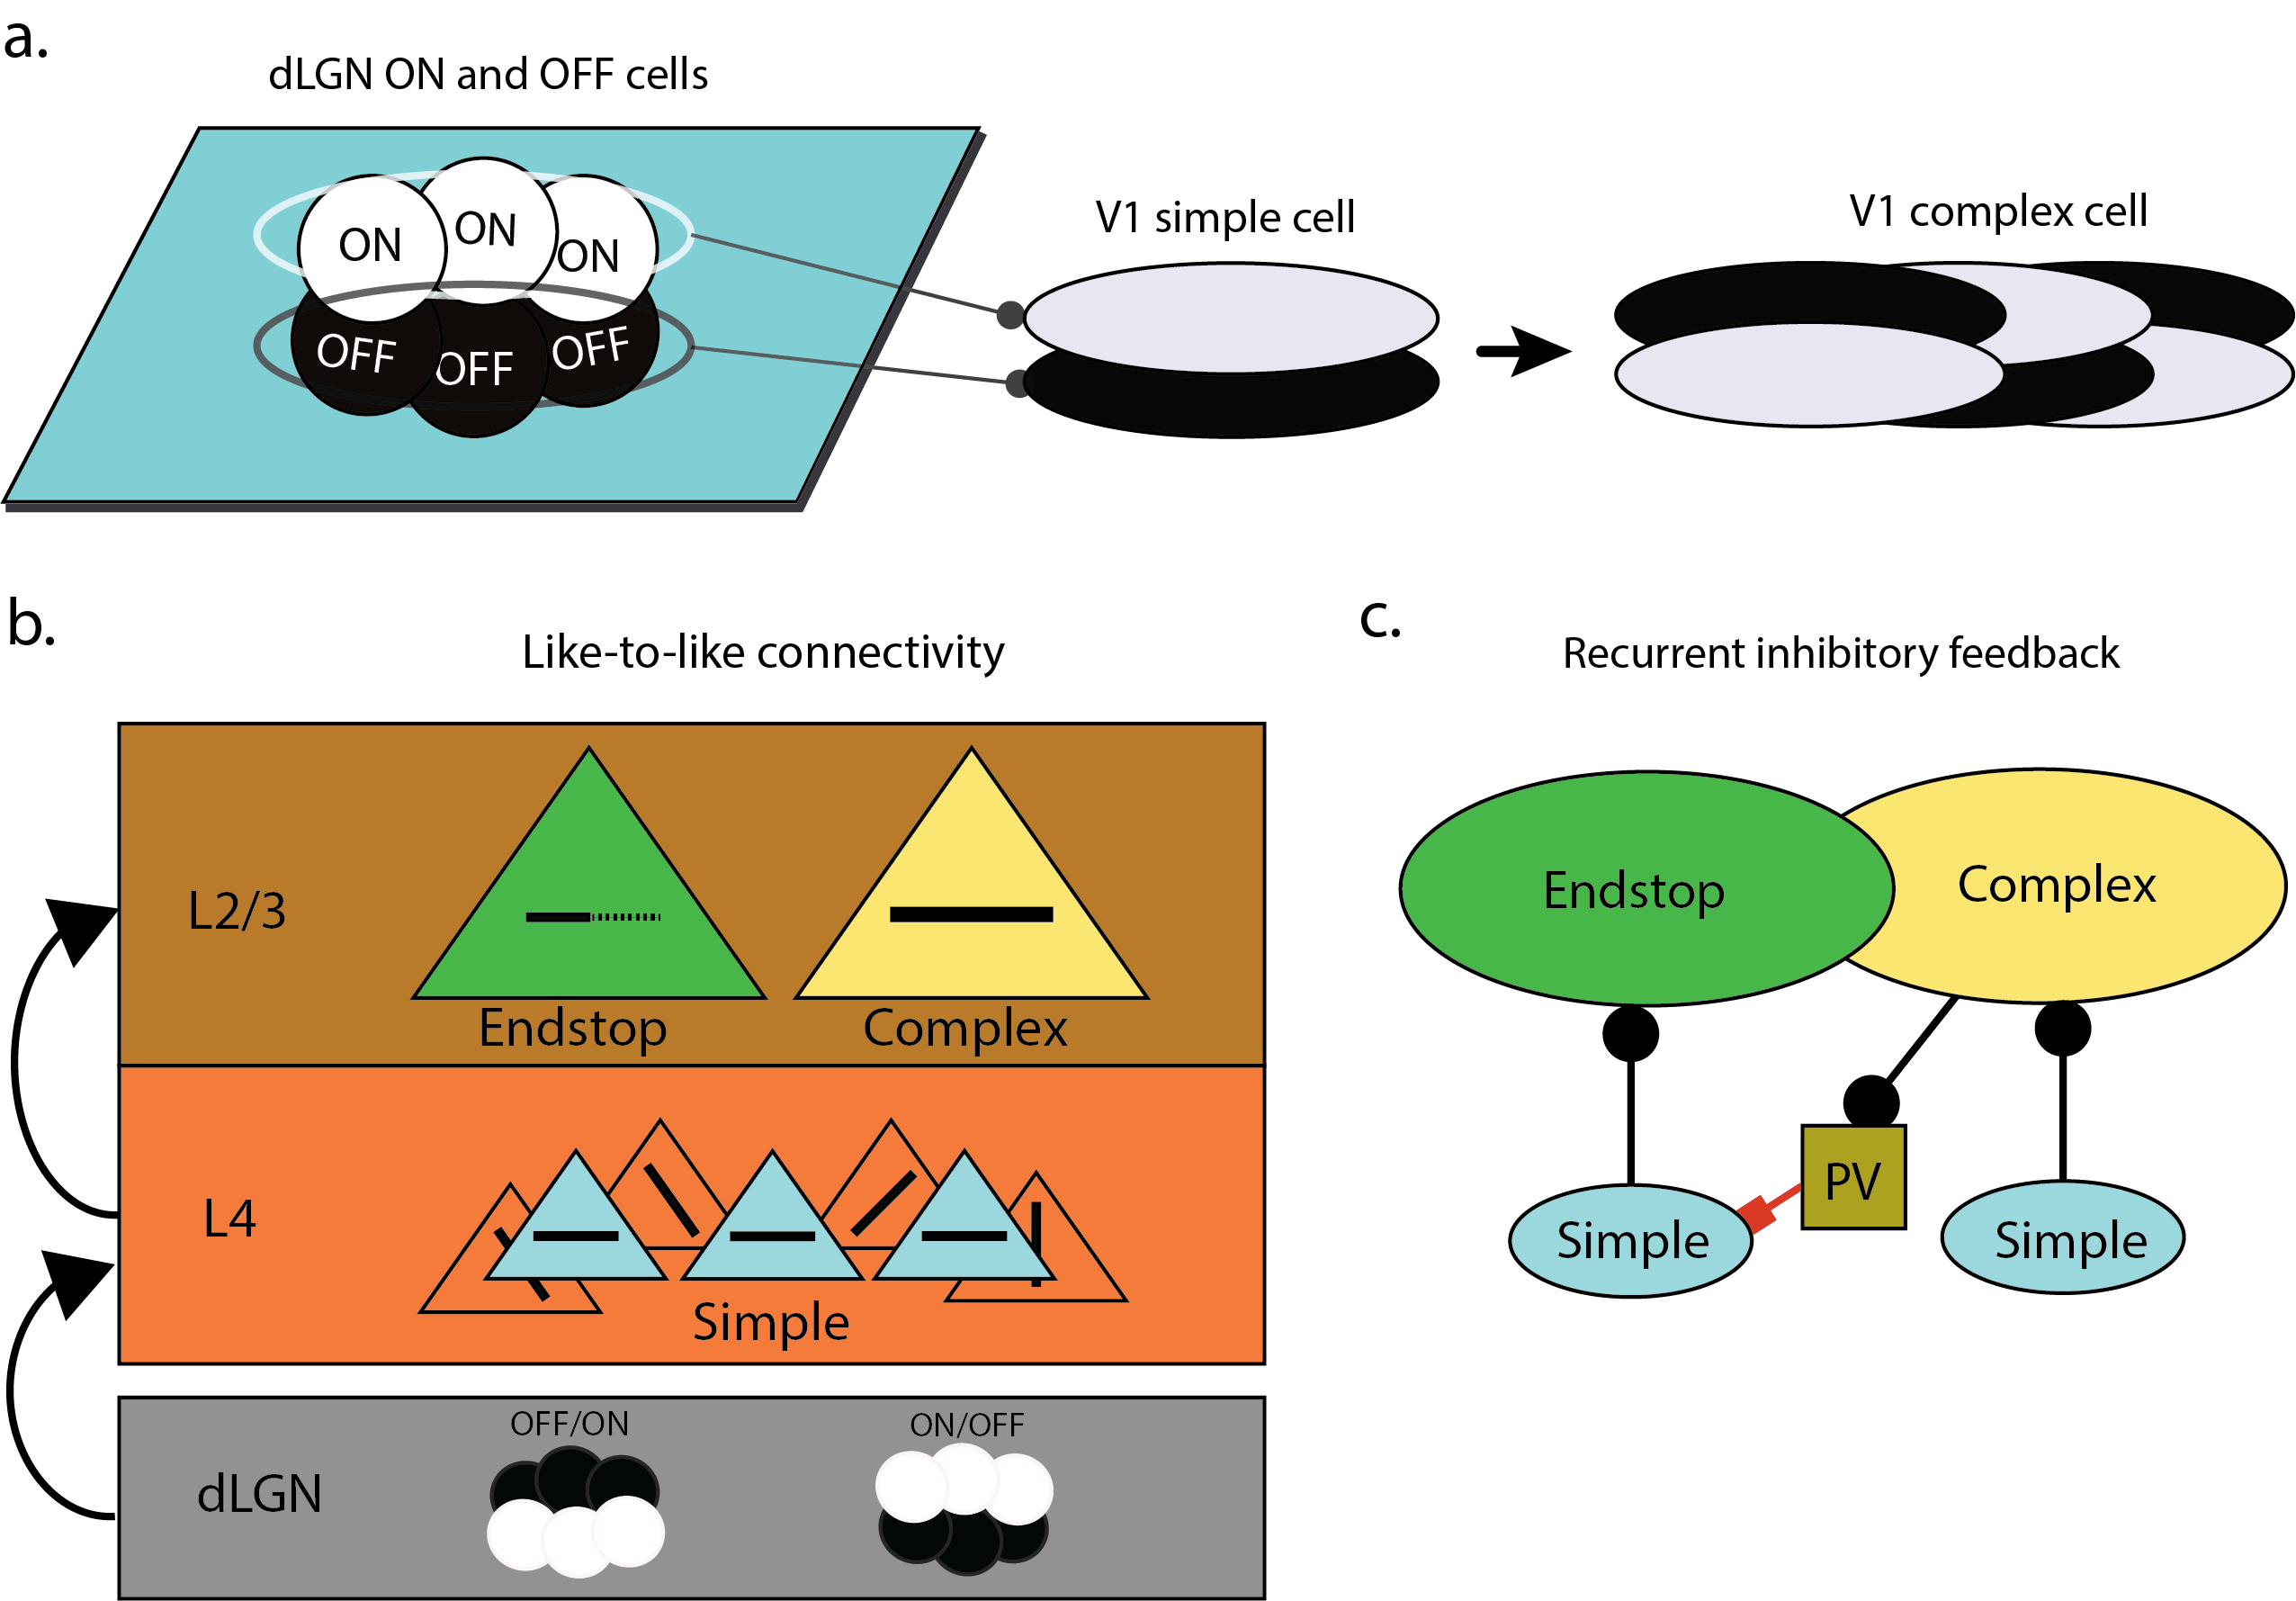
\includegraphics[width=1.0 \textwidth]{adjusted_figures/LIF_Overview_Receptive_Field_Methods.png}
  \caption{a. The dLGN ON and OFF cells that converge with a spatial offset onto a simple cell, creating a simple filter that responds to edges. Combining multiple simple cells with overlapping ON and OFF fields creates a complex cell. The complex cells, due to their overlapping subfields are not dependent on stimulus polarity and are phase invariant. b. A diagram showing the hierarchical complexity of cells that are connected based on their orientation tuning. The green endstopped cell is illustrated by a dotted line end, showing that an extended line end will result in a decreased firing rate. c. Shows how a particular endstopped microcircuit is made. Population of simple cells converge onto the endstop and complex cell to give them feedforward input, however if a line would extend over the endstopped receptive field, stimulating the complex cell. A recurrent inhibitory feedback loop would inhibit the simple population that is responsible for the endstopped cell's drive and firing will decrease. }
  \label{fig:LIF_Overview}
\end{figure}


\subsection{dLGN during stimulus presentation}
The first relay station in the visual pathway is the dorsal Lateral Geniculate Nucleus (dLGN), which receives input from the retina and transmits visual information to the primary visual cortex (V1) for further processing. The dLGN processes visual stimuli through two distinct pathways: the ON and OFF pathways, which respond to increases and decreases in light intensity, respectively. These pathways are essential for encoding contrast and edge information in visual scenes, providing the initial processing steps that shape the neural representation of visual stimuli. To simulate the dLGN's response to visual stimuli, we used the Brain Modeling Toolkit (BMTK) to construct a network of dLGN cells and present monochromatic greyscale images to the network. The BMTK provides a flexible framework for building and simulating neural networks, allowing us to define the spatial arrangement of dLGN cells, their receptive fields, and their connectivity patterns. By presenting visual stimuli to the dLGN network, we can effectively simulate the translation of light input into neural signals, creating the first layer for contrast detection in the visual system. Since we are interested in contrast, which is encoded in V1 rather than color, only monochromatic greyscale stimuli were shown. To transform this input array into neural signals, the dLGN was simulated as a linear-non-linear Poisson cascade model. First, visual input within the space of the receptive field of the LGN cell is convolved with a linear filter. Then a nonlinear function is applied to the output of the previous linear filter, giving the neuron's instantaneous spike rate as its output. Finally, this firing rate generates spikes according to an inhomogeneous Poisson process \autocite{moskovitzComparisonDeepLearning2018}. The current dLGN model consists of two unit types, ON and OFF surround cells, optimized to closely mimic mammalian thalamic cells. The ON and OFF cells of the LGN converge on a layer of simple cells, effectively simulating layer 4 (L4) of V1 (Figure \ref{fig:LIF_connectivity}a). This dual pathway of ON/OFF cells is essential for the initial segregation of visual information, setting the stage for more complex edge detection and contrast processing within higher cortical areas. We analyzed spiking features in response to static images. Therefore, we focused on modeling ON and OFF cells to have a predominantly sustained responses (sON and sOFF). We used the model templates in our node configuration to implement these cells in our network. The parameters for these cells were set based on values derived from electrophysiological recordings from the mouse dLGN, as reported by \textcite{durandComparisonVisualResponse2016} and \textcite{billehSystematicIntegrationStructural2020}.

\begin{figure}[H]
  \centering
  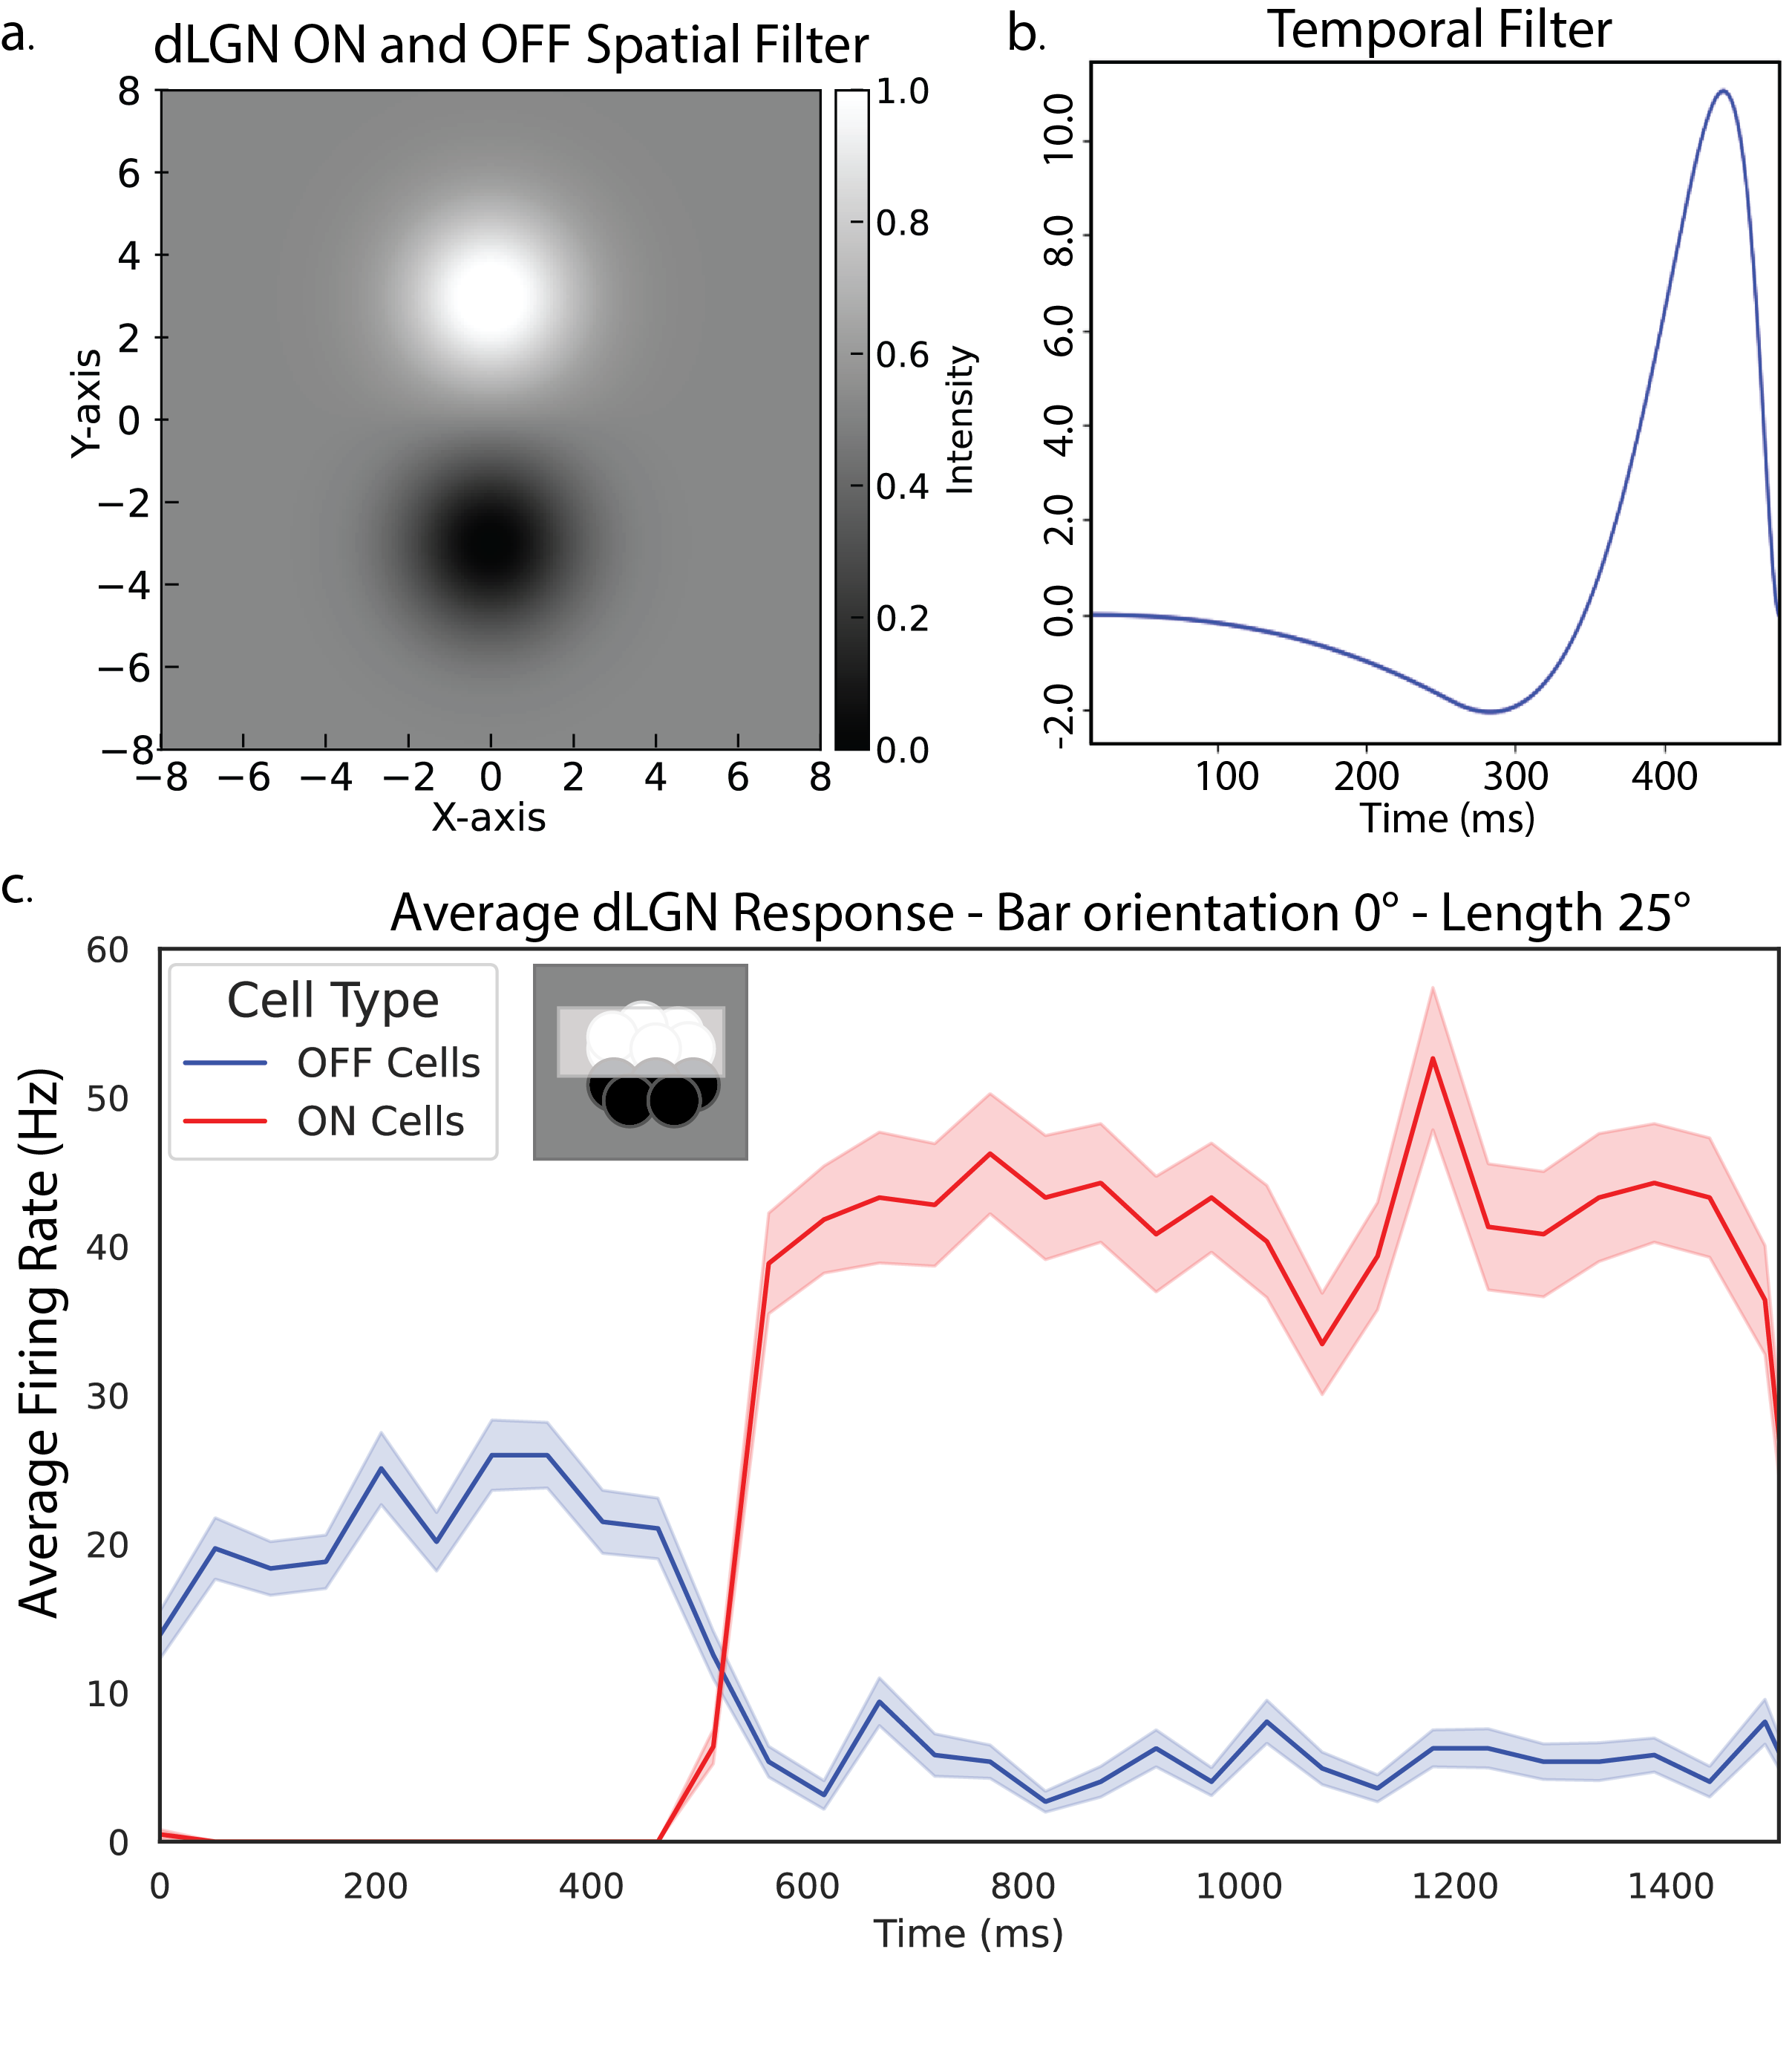
\includegraphics[width=1.0 \textwidth]{figures/lgn_response_fig.png}
  \caption{a. The ON and OFF spatial filters used as input to V1 simple cells. The ON and OFF filters are two inverted gaussian functions that are sensitive to bright and dark input, respectively. b. Each filter also has a temporal filter that dictates how the response changes through time. c. The ON and OFF response to a bar that is completely stimulating the ON cells as well as some minor stimulation to the OFF cells. The stimulus is a bar with a length of 25 visual degrees and is completely horizontal with a rotation of 0 degrees. All stimuli presented to the dLGN were monochromatic and could be represented by either ON or OFF cells.}
  \label{fig:LIF_connectivity}
\end{figure}

\textbf{LGN and V1 parameters} For the spatial filtering of the receptive fields, we employed a Gaussian filter characterized by its spatial size and rotation. The default spatial size was set to 5.0 spatial degrees for both rows and columns, with a rotation of 0.0 degrees. The temporal filtering was managed using a double cosine filter. The parameters for this filter included weights, kpeaks, and delays. The weights parameter controlled the amplitude of the two peaks in the cosine filter, with the first value being greater than the second (weights[0] > weights[1]). The kpeaks parameter determined the spread of the peaks, ensuring the second peak had a greater spread than the first.

The delays parameter controlled the timing of the peaks, with delays[0] setting the delay for the first, larger peak and delays[1] setting the delay for the second, smaller peak. A smaller value for delays[0] resulted in a quicker initial response to brightness changes, while a larger value meant a slower initial response. Similarly, delays[1] determined how quickly the secondary response occurred, with smaller values indicating quicker secondary responses and larger values indicating slower ones. By carefully setting these parameters, we ensured that the LGN cells accurately modeled the sustained neural responses to both ON and OFF input necessary for our study.

\begin{table}[H]
  \centering
  \caption{Parameters and Weights for LGN and V1 Cells}
  \begin{tabular}{lll}
  \toprule
  \textbf{Cell Type} & \textbf{Parameter} & \textbf{Description} \\
  \midrule
  \multirow{4}{*}{LGN} 
      & Optimized weight      & (7, -1) \\
      % & Parameter bounds   & P \\
      & Delays   & (0, 0) \\
      & K-peaks   & (30, 55) \\
  \midrule
  \multirow{7}{*}{V1} 
      & External current         & 0.0 nA \\
      & Membrane time constant        & 44.9 ms \\
      & Membrane capacitance          & 239.0 pF \\
      & Refractory period       & 3.0 ms \\
      & Resting potential          & -78.0 mV \\
      & Threshold potential         & -43.0 mV \\
      & Reset potential      & -55.0 mV \\
  \bottomrule
  \end{tabular}
\end{table}

\subsection{Orientation Selectivity in V1}
Our study aimed to achieve orientation selectivity in V1 simple cells by strategically connecting LGN cells to them using elliptical receptive fields. Specifically, we designed each simple cell in V1 to have a receptive field composed of two distinct elliptical regions: one for ON and one for OFF responses. These ellipses were positioned relative to each other and oriented along a specific angle, allowing the V1 cells to sample input selectively from ON and OFF LGN cells. To implement this, we first defined the receptive field for each V1 simple cell by setting the parameters of the ellipses. Each ellipse had a specific orientation, which was determined by the angle of its major axis, reflecting the preferred orientation of the V1 cell. The separation between the centres of the ON and OFF ellipses was carefully specified to ensure that these regions were spatially distinct but aligned according to the desired orientation. This separation allowed the ON and OFF regions to be positioned, so they could selectively sample from the respective ON and OFF LGN cells.

\noindent Connections from the LGN cells to the V1 simple cells were established using a selective connection rule implemented through a connection function. This function determined whether an LGN cell's position fell within the bounds of the ON or OFF ellipse of a given V1 cell. For each LGN cell, the function checked if the cell's position was within the elliptical boundary using a mathematical condition that defines whether a point lies inside an ellipse. This condition was based on the ellipse's centre, axes, and orientation, allowing precise determination of the inclusion of LGN cells within the receptive fields of the V1 cells. Once an LGN cell was identified as being within the receptive field of a V1 cell, synaptic connections were established with specific weights and delays. These synaptic parameters were carefully tuned to reflect the physiological properties of synaptic transmission observed in biological systems. The synaptic weights determined the strength of the input from the LGN cell to the V1 cell, while the delays accounted for the time taken for the signal to travel between the two cells. The network construction involved creating a V1 network with simple cells characterized by their orientation, positions, and receptive field parameters, such as the separation between ellipses, the radius, and the aspect ratio of each ellipse. The positions of the V1 cells were generated within a specified spatial grid to simulate the realistic arrangement of neurons in the visual cortex. Similarly, the LGN cells were distributed across a spatial grid with their positions randomly generated within defined bounds, reflecting the natural variability in the spatial distribution of these cells. The selective connection rule played a crucial role in achieving orientation selectivity. The rule iterated over all possible LGN sources for each V1 target, checking for inclusion within the ellipses and establishing connections accordingly. This process ensured that each V1 simple cell received input from a specific subset of LGN cells aligned with its receptive field configuration. By connecting each V1 cell to a well-defined set of ON and OFF LGN cells, the V1 cells could respond preferentially to specific orientations of visual stimuli. Through this method, elliptical receptive fields with distinct ON and OFF regions enabled the V1 simple cells to become orientation-selective. The careful design of the spatial arrangement of the ellipses, combined with the selective connection rules, ensured that the V1 cells exhibited orientation selectivity similar to that observed in biological visual systems. This approach provided a robust model for studying the mechanisms of orientation selectivity and the role of specific LGN inputs in shaping the response properties of V1 neurons.

\begin{figure}[H]
    \centering
    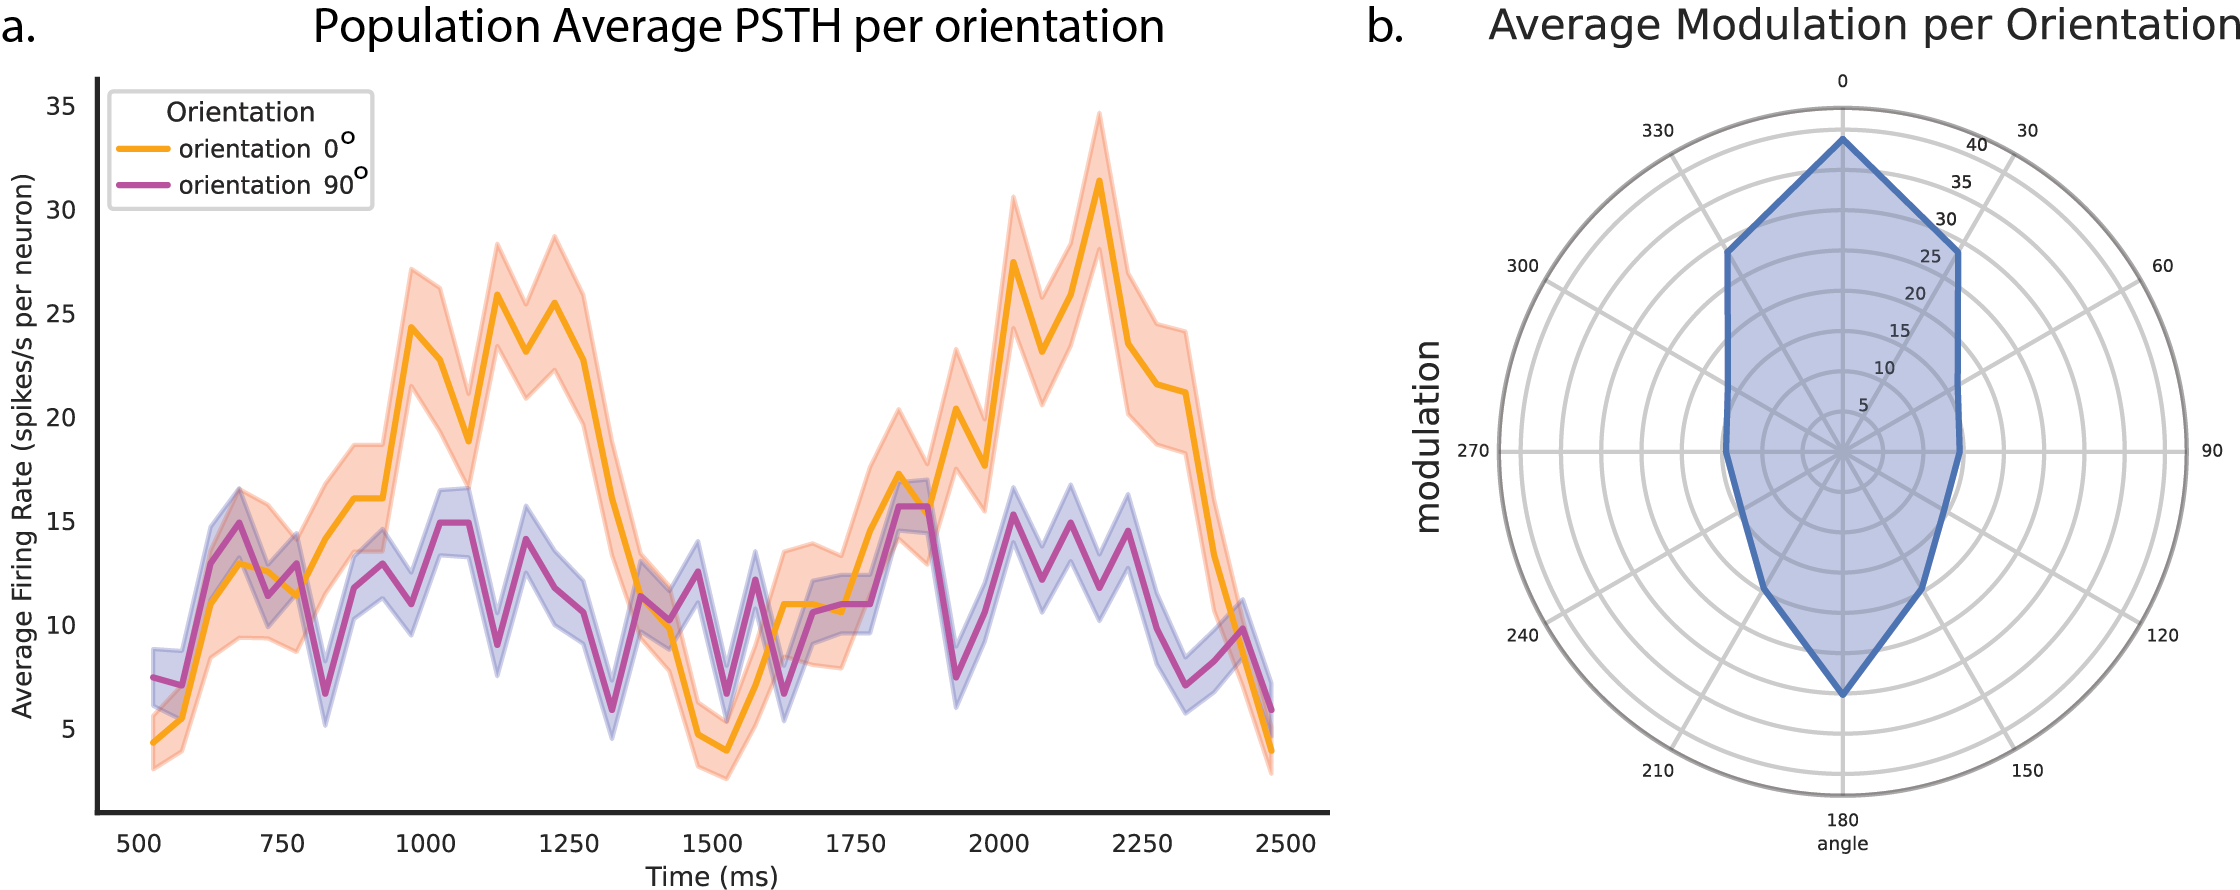
\includegraphics[width=1.0 \textwidth]{figures/figure_simple_orientation_tuning.png}
    \caption{a. The average orientation tuning of a population of simple cells. The input was a drifting grating with different orientations. In orange a horizontal drifting grating with 0 degrees rotation, and in purple a drifting grating with a 90 degree rotation. Simple cells show a phase sensitivity demonstrated by the two peaks, in which the cell receives no input from the dLGN. b. A polar plot showing the average firing modulation per orientation, showing that the cells respond to 0 and 180 degrees rotated stimuli.}
    \label{fig:simple cell orientation tuning}
\end{figure}

\subsection{Polarity Invariance of Complex Cells.}
Subsequently, complex cells are created by strategically connecting these simple cells. The process began by connecting LGN cells to V1 simple cells using elliptical receptive fields and then by combining simple cells to form complex cells; we ensured phase invariance and enhanced orientation selectivity. To create a phase invariant complex cells a small number of retinotopically aligned simple cells were connected to achieve overlapping ON/OFF and OFF/ON receptive fields. The converging simple cells all had the same preferred orientation but different spatial phases creating a single complex cell. The selective connection rule played a crucial role in this process. The rule iterated over all possible simple cell sources for each target complex cell, checking for alignment in orientation and differences in phase. Synaptic connections were established between the simple cells and the complex cell, ensuring that the complex cell received inputs from a diverse set of simple cells. This convergence allowed the complex cell to respond to a range of spatial phases of a given orientation, thereby achieving phase invariance.

In the code implementation, complex cells were created by defining their receptive fields and connecting them to simple cells using a similar selective connection rule. The positions of complex cells were generated within a specified spatial grid, and their receptive fields were aligned with the preferred orientations of the contributing simple cells. The connection rule ensured that each complex cell received input from multiple simple cells with the same orientation preference but different phase preferences. This was accomplished by iterating over all potential simple cell sources for each target complex cell, establishing connections based on the orientation and phase alignment. Through this method, elliptical receptive fields with distinct ON and OFF regions enabled V1 simple cells to become orientation-selective. By combining these simple cells to form complex cells, we achieved phase invariance, allowing complex cells to respond robustly to a given orientation regardless of the spatial phase of the input. The careful design of the spatial arrangement of the ellipses, the selective connection rules, and the convergence of simple cells onto complex cells ensured that the V1 network exhibited properties similar to those observed in biological visual systems. This approach provided a robust model for studying the mechanisms of orientation selectivity, phase invariance, and the role of specific LGN and simple cell inputs in shaping the response properties of V1 neurons.


\begin{figure}[H]
    \centering
    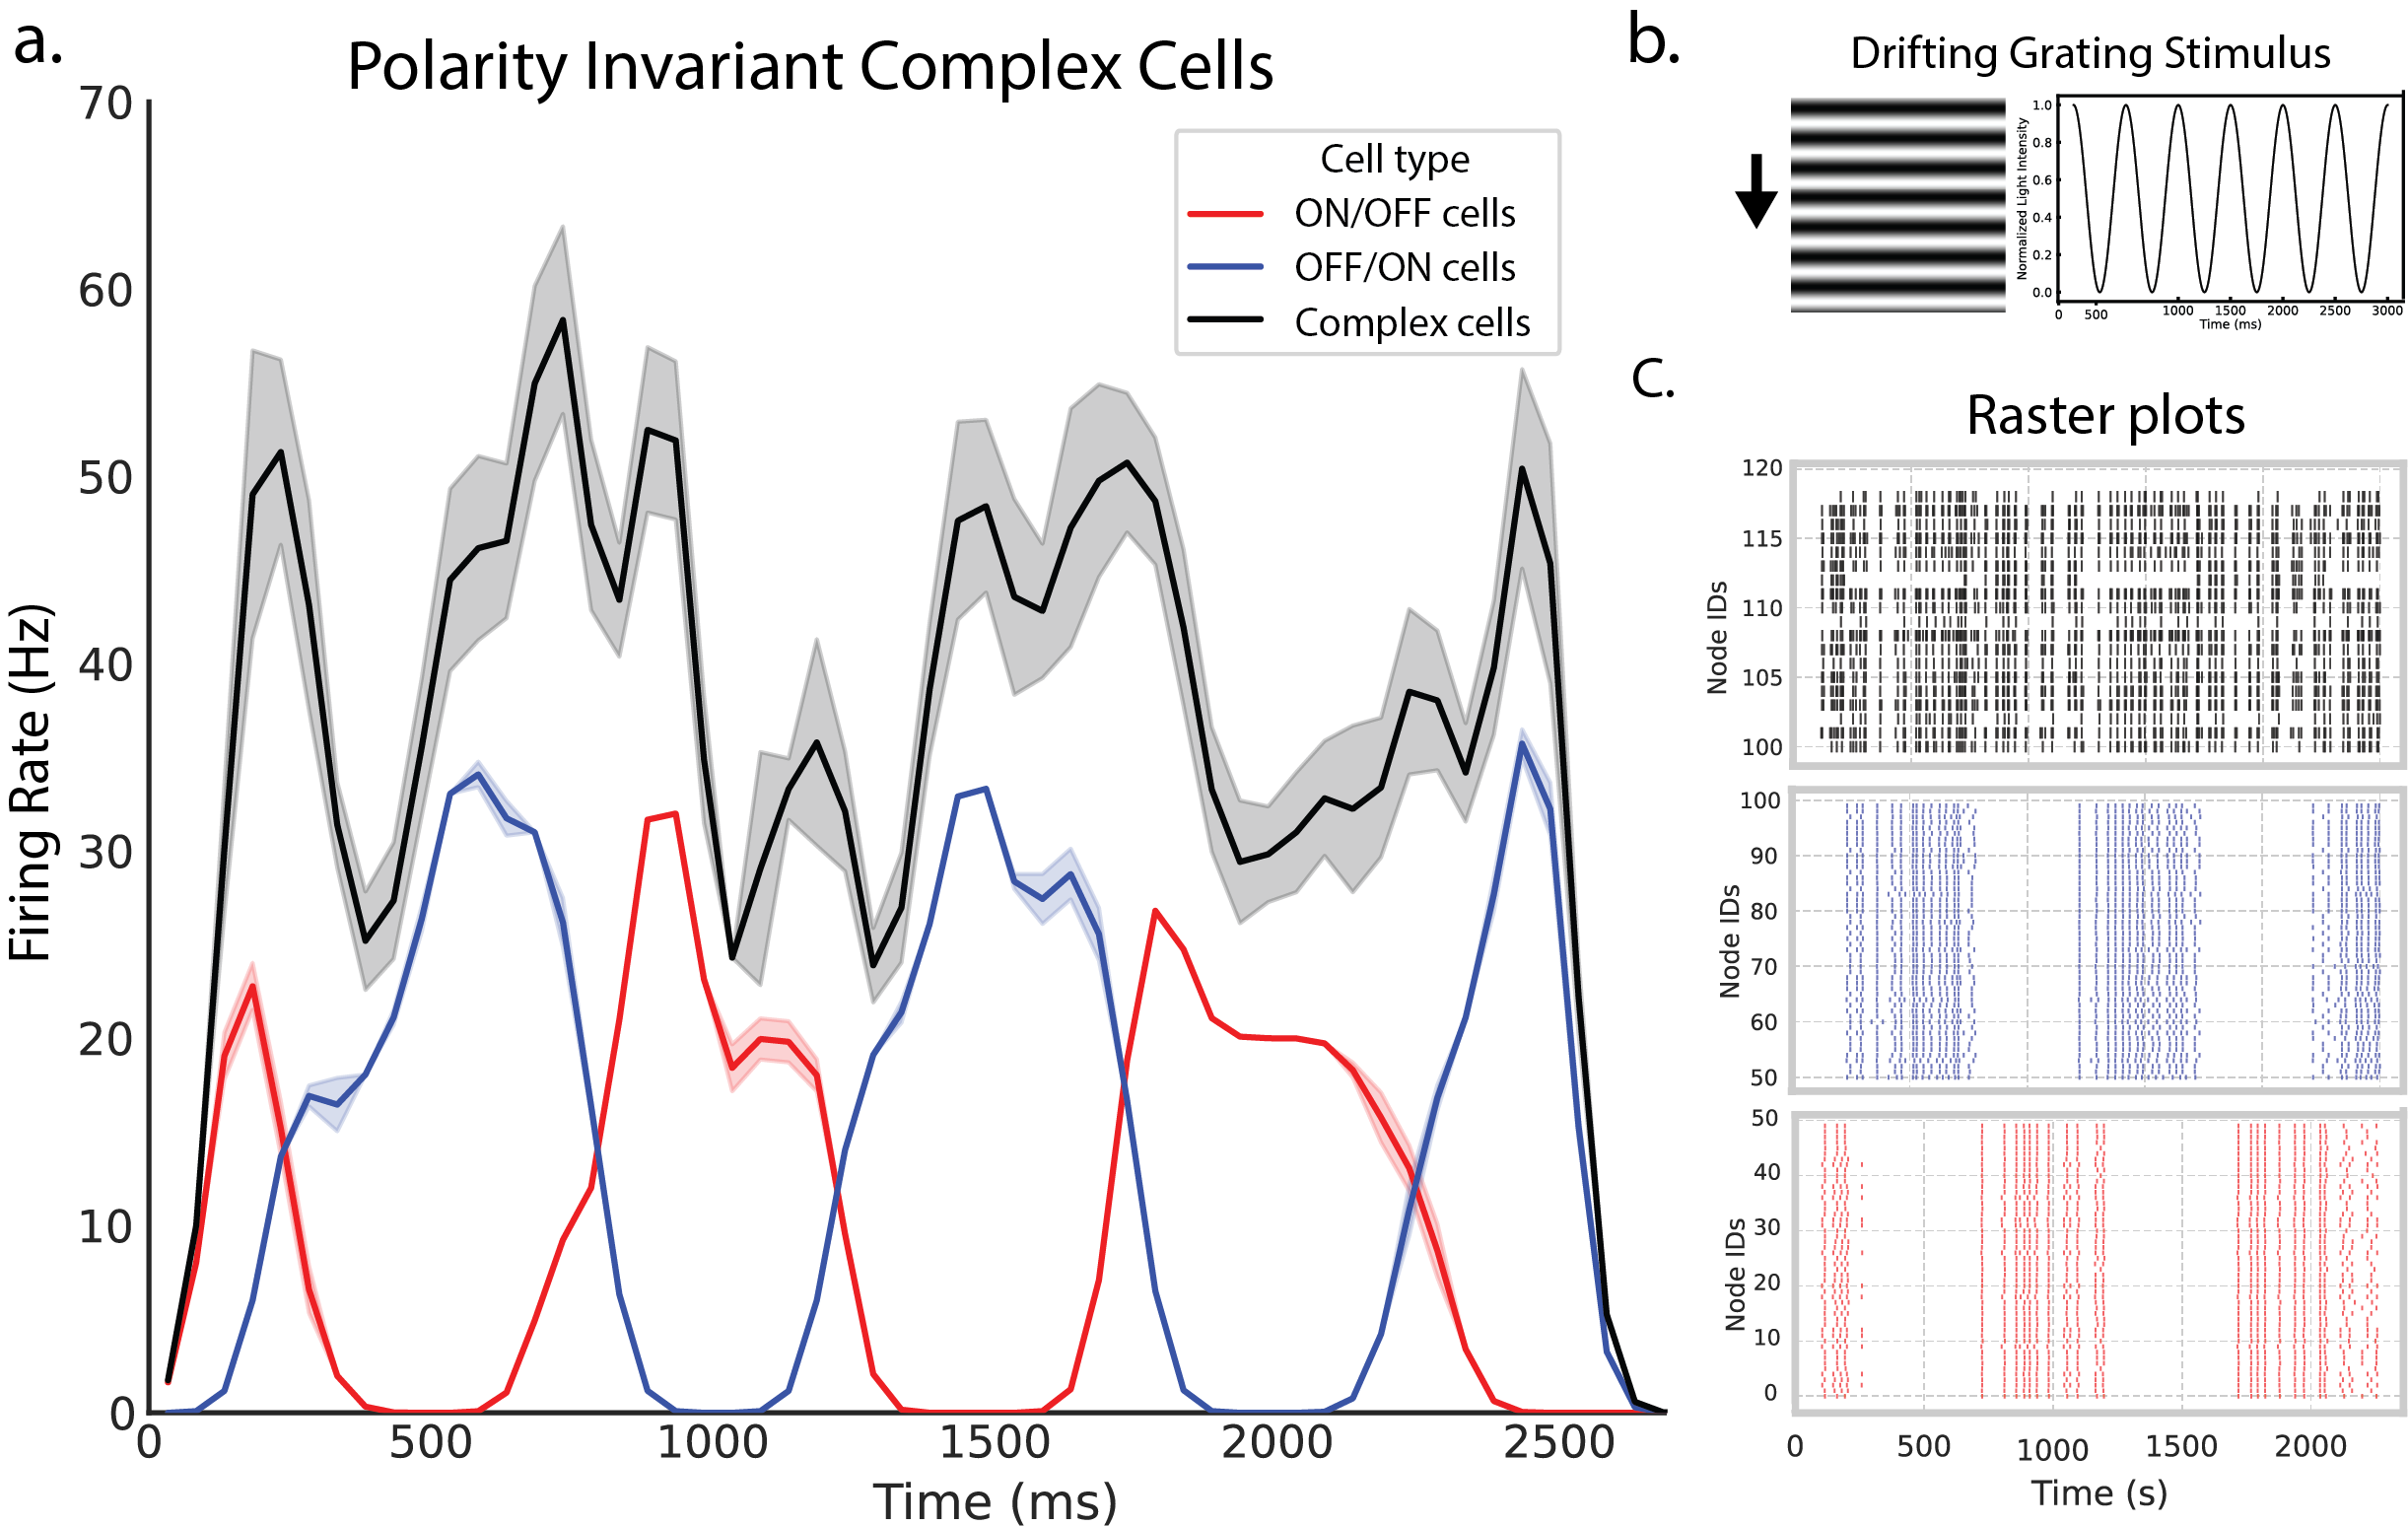
\includegraphics[width=1 \textwidth]{figures/complex_invariance_figure.png}
    \caption{a. Simple and complex cells responses to a horizontal drifting grating. ON/OFF simple cells are shown in red with an offset phase from the OFF/ON cells. The black complex cells do not exhibit the same phase sensitive. b. The drifting grating stimulus that was presented to the model. c. The raster plots also illustrate the phase sensitivity of the simple cells and how the complex cell has a stable firing to a constantly fluctuating input.}
    \label{fig:polarity invariance}
\end{figure}

\subsection{Recurrent feedback underlying endstopping.}
In the initial phases of the current model, an attempt was made to create endstopping by strictly combining ON and OFF fields in an excitatory manner. The idea was to spatially offset specific simple ON and OFF fields relative to each other, modeling the inhibitory subfield of an endstopped cell with an OFF field and the excitatory subfield with an ON field. While this method reduced the firing rate, it did not achieve a nulled spiking rate. Therefore, in subsequent methods, we first integrated the simple ON/OFF streams into complex cells before introducing spatial relationships between cells. Additionally, to create orientation-selective and phase-invariant cells that exhibit endstopping behavior, we used recurrent activation of inhibitory cells to model this critical feature of visual processing. This process began with the projection of simple cells into complex cells. Specifically, simple cells with orientation-selective receptive fields were connected to complex cells that integrated inputs across different spatial phases, thus achieving phase invariance. The next step involved a laterally displaced complex cell. This neighbouring complex cell then projected to a population of inhibitory interneurons that was connected to the original simple cell population \hyperref{fig:LIF_Overview}. This displacement was crucial as it introduced a spatial offset between the excitation source and the location where inhibition would be applied, mimicking the spatial dynamics observed in cortical circuits. The inhibitory interneurons targeted by these projections played a key role in modulating the activity of the simple cells. Once activated by the complex cells, the inhibitory cells provide feedback to the simple cells positioned in the retinotopically overlapping area of the original complex cells. This feedback loop was designed to suppress the activity of the simple cells when a stimulus extended beyond their receptive field. In more detail, as a line or bar stimulus moved across the receptive field of a simple cell and extended beyond it, the laterally displaced complex cell would activate the inhibitory interneurons. These interneurons, in turn, would inhibit the simple cells, thereby reducing their firing rate. This rapid inhibition is a hallmark of endstopping, where the neuron's response is curtailed when a stimulus exceeds the optimal length within its receptive field. The introduction of this recurrent feedback mechanism was essential for creating endstop cells, which are specialized for detecting the endpoints of lines and bars. Endstop cells are known for their ability to signal the presence of corners, line ends, and other salient features in the visual field, making them critical for complex shape and motion perception. By implementing this feedback loop, the model could replicate the rapid decline in firing rate that characterises endstopping, providing a more accurate and nuanced representation of visual processing as seen in the primary visual cortex. This approach highlights the importance of inhibitory feedback in fine-tuning the responses of neurons to visual stimuli, ensuring that the network could adapt to varying stimulus lengths and shapes. The recurrent feedback to inhibitory cells not only enhanced the functional properties of the model but also added a layer of biological realism by incorporating mechanisms observed in actual neural circuits. Through this detailed modelling, the network was able to exhibit advanced visual processing capabilities, closely mirroring the behaviour of endstop cells found in the visual cortex.

%ToDo change exc inh etc. to population names
\begin{table}[h]
  \centering
  \caption{Connection Weights in the LIF endstop Circuit}
  %\label{tab:weights}
  \begin{tabular}{@{}llc@{}}
      \toprule
      \textbf{From} & \textbf{To} & \textbf{Weight} \\ \midrule
      Excitatory (e) & Excitatory (e) & 0.8 \\
      Excitatory (e) & Inhibitory (i) & 2.5 \\
      Inhibitory (i) & Excitatory (e) & -3.0 \\ \bottomrule
  \end{tabular}
\end{table}

\subsection{Population activity and illusory contour representation.}
In order to investigate the generation of illusory contour in the visual cortex, we used population activity models to abstract the endstopping responses of V1 neurons to visual stimuli as presented in our LIF model in a more tractable form. The population models allowed us to recreate the interlaminar endstopping microcircuits by treating each cell type as a specific population and study how multiple endstopping microcircuits collectively encoded the presence of illusory contours in a specific retinotopic coordinate of the visual field. This way we still captured the dynamic interactions between simple, complex, endstopping, and inhibitory interneurons, while providing a network of which the activity could be further integrated in a higher visual cortical area such as lateromedial cortex (LM), the second visual area in the mouse. In turn, this allowed us to examine how higher level visual feedback could provide information for V1 to induce an illusory filling in mechanism between retinotopic coordinates. Thus, abstracting the LIF model into a population model allowed for a more comprehensive view of how V1 processes visual information in the case of possible occlusion and how an illusory response can be generated to particular stimulus configurations.

\subsubsection{Overview of the population model.}
This text should describe the connectivity patterns used to shape the population model, the parameters used to define the neural dynamics, and the overall structure of the model. It should also explain how the model was used to simulate the generation of illusory contours in the visual cortex and how the results were interpreted to gain insights into the neural mechanisms underlying this phenomenon.
%ToDo describe connectivity patterns used to create population model.


\begin{figure}[H]
  \centering
  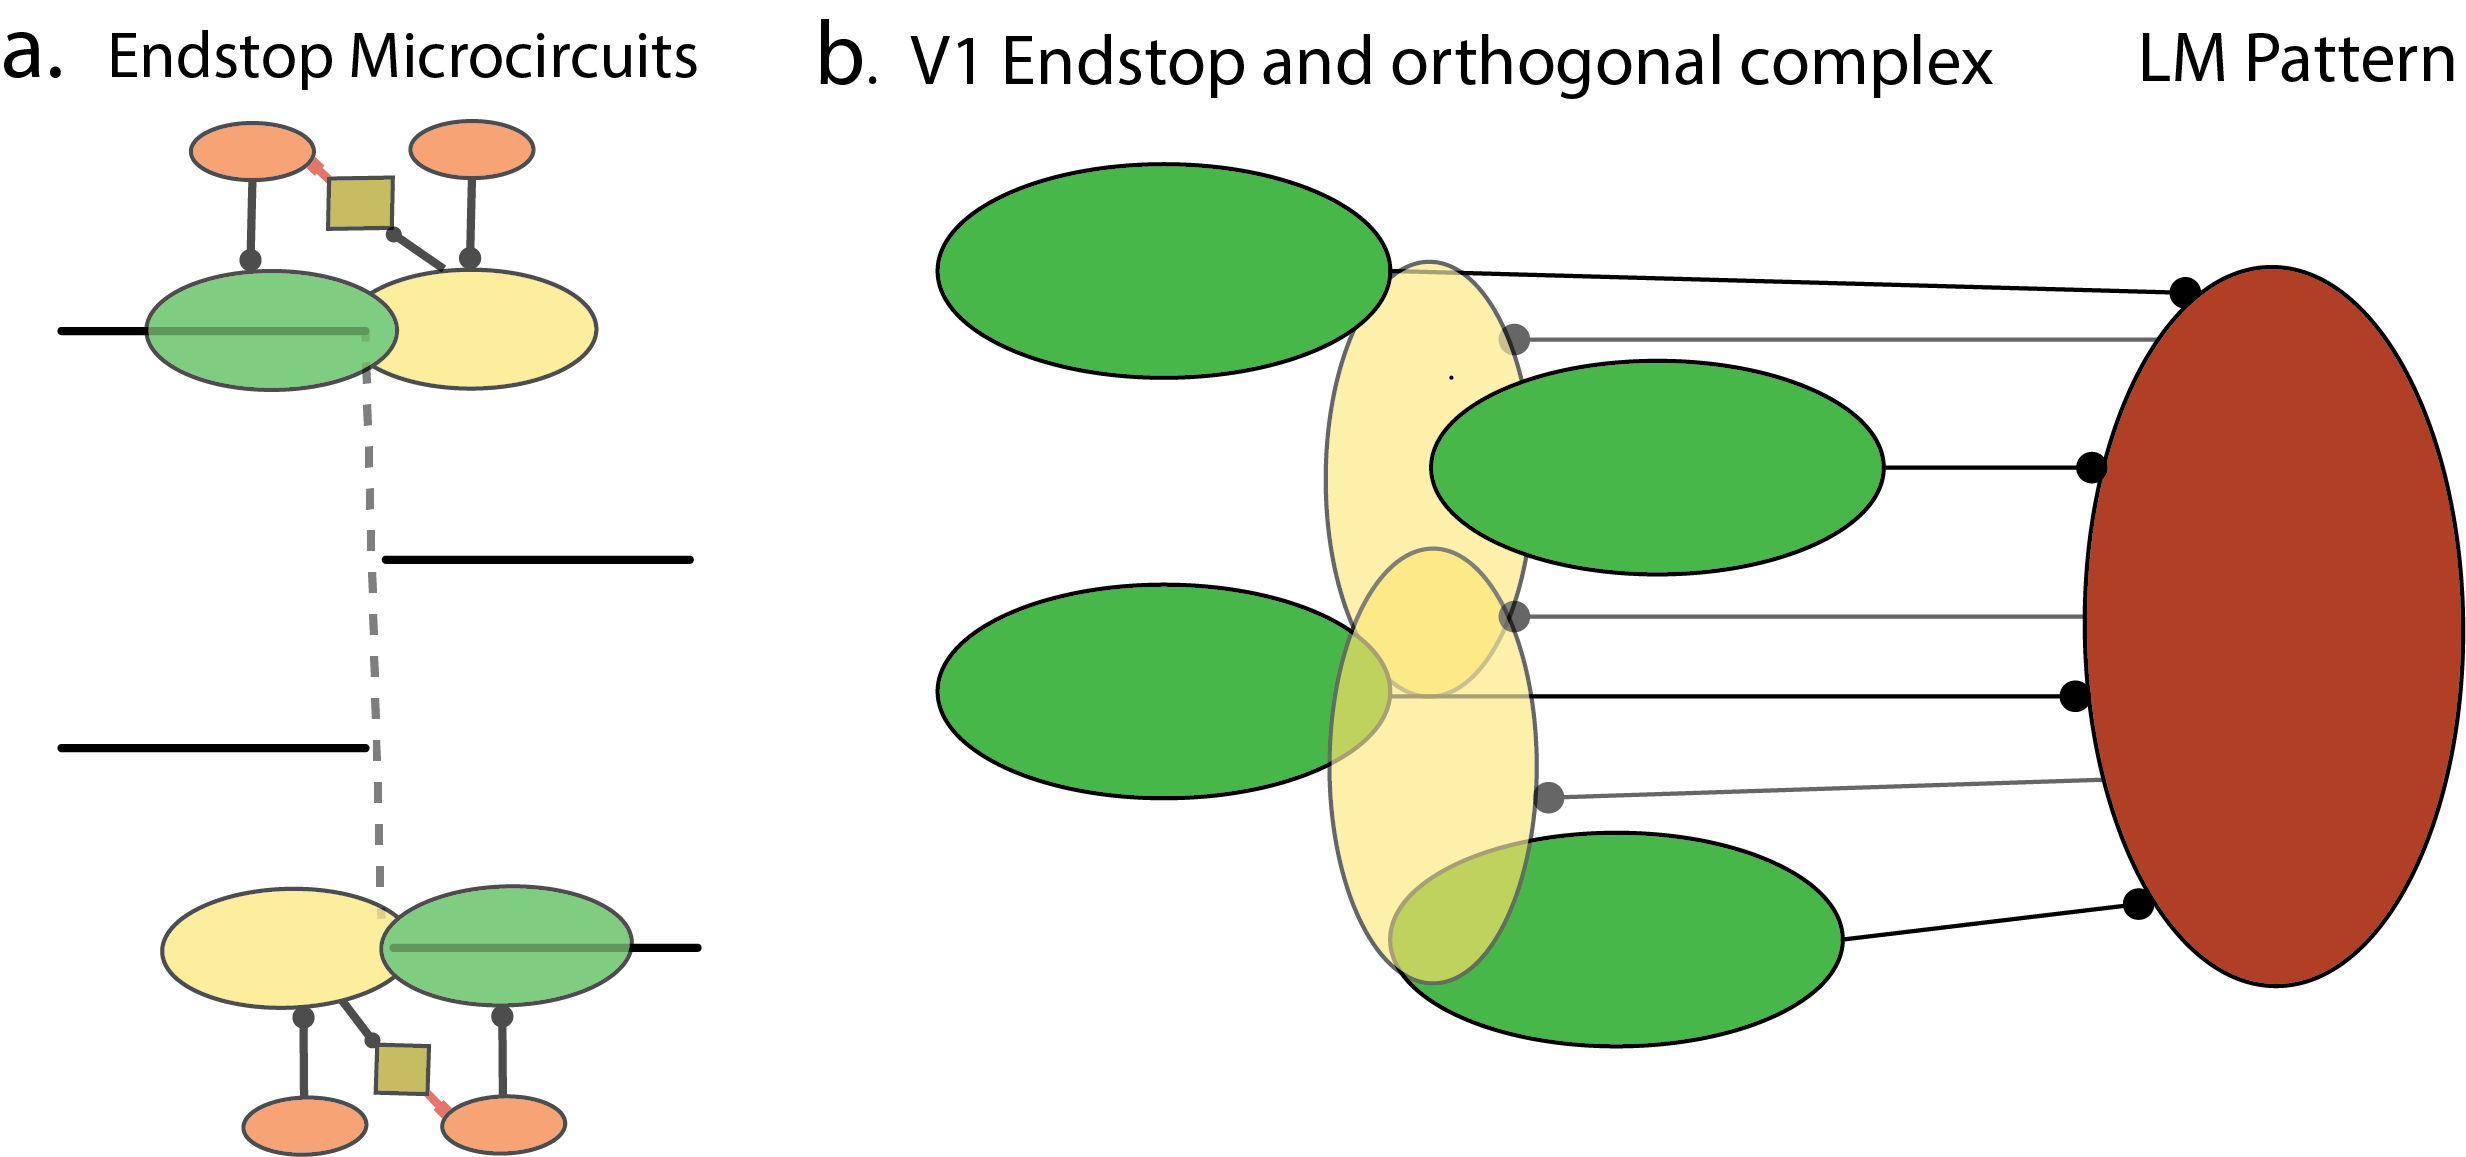
\includegraphics[width=1 \textwidth]{adjusted_figures/illusory_filling.png}
  \caption{a. The endstopped microcircuit illustrated on top of horizontal abutting grating illusion inducers. The elements that make up the microcircuit share the same retinotopic coordinates. b. If all 4 of the endstopped cells are active they fire intensely enough to activate a higher visual pattern cell in LM, which integrates these input and projects feedback onto orthogonally tuned complex cells. This way an illusory contour is locally represented through the integration of local endstopped signals.}
  \label{fig:illusory_filling}
\end{figure}


\subsubsection{PyRates Library and population parameters.}
In our study, we employed a Wilson and Cowan neural mass model using the PyRates library to simulate neural dynamics. This model helps us understand how groups of neurons interact with each other over time. It consists of several key components and parameters that we will explain in detail.

First, we define an operator called the synaptic excitation operator (\texttt{se\_op}). This operator uses a sigmoid function to model the process of synaptic excitation, which is how neurons get excited and send signals. The equation for this operator is:
\[
m = \operatorname{sigmoid}(s \cdot (r_{\mathrm{in}} + r_{\mathrm{ext}} - \theta)) - \operatorname{sigmoid}(-s \cdot \theta),
\]
where \( m \) represents the output signal from the neuron. The term \(\operatorname{sigmoid}\) is a mathematical function that smoothly limits the output between 0 and 1, mimicking the neuron's firing rate. The parameter \( s \) controls the steepness of the sigmoid curve and is set to 1.0, meaning it defines how quickly the neuron responds to input. The parameter \(\theta\) is a threshold set to 2.0, which the input must exceed for the neuron to start firing significantly. The inputs \( r_{\mathrm{in}} \) and \( r_{\mathrm{ext}} \) represent signals coming from other neurons and external sources, respectively, and both are initially set to 0.0.

We also have a variation called the synaptic inhibition operator (\texttt{si\_op}). This operator works similarly but models inhibitory signals, which reduce neuron activity. Its equation is similar, but with different parameters: \( s \) is set to 2.0, making the response steeper, and \( \theta \) is set to 2.5, meaning a higher threshold for inhibition.

Next, we describe the rate operator (\texttt{rate\_op}). This operator models the rate of change in neural activity over time using the differential equation:
\[
r' = \frac{-r + (1.0 - k \cdot r) \cdot m}{\tau}.
\]
Here, \( r \) is the current activity level of the neuron, initially set to 0.0. The parameter \( k \) is set to 1.0 and influences how the neuron's activity decreases over time. The term \( \tau \) represents the time constant set to 10.0, which defines how quickly the neuron activity responds to changes. The input \( m \) is the signal calculated by the excitation or inhibition operators.

To model neural populations, we use node templates. The excitatory population node template (\texttt{exc\_pop}) combines the rate operator and the synaptic excitation operator to represent a group of excitatory neurons, which promote activity in the network. Conversely, the inhibitory population node template (\texttt{inh\_pop}) combines the rate operator and the synaptic inhibition operator to represent a group of inhibitory neurons, which suppress activity in the network.

Circuit templates define the network structure of the model. The Wilson-Cowan circuit template (\texttt{WC}) consists of two nodes: an excitatory population (\texttt{e}) and an inhibitory population (\texttt{i}). The parameters used in the model are summarized in Table~\ref{tab:parameters}.

\begin{table}[h]
    \centering
    \caption{Parameters of the Wilson-Cowan Neural Mass Model}
    \label{tab:parameters}
    \begin{tabular}{@{}lll@{}}
        \toprule
        \textbf{Parameter} & \textbf{Description} & \textbf{Value} \\ \midrule
        \( s \) & Steepness of the sigmoid curve (excitation) & 1.0 \\
        \( \theta \) & Threshold for excitation & 2.0 \\
        \( r_{\mathrm{in}} \) & Input from other neurons & 0.0 \\
        \( r_{\mathrm{ext}} \) & External input & 0.0 \\
        \( s \) (inhibition) & Steepness of the sigmoid curve (inhibition) & 2.0 \\
        \( \theta \) (inhibition) & Threshold for inhibition & 2.5 \\
        \( r \) & Current activity level & 0.0 \\
        \( k \) & Decay parameter for activity & 1.0 \\
        \( \tau \) & Time constant & 10.0 \\ \bottomrule
    \end{tabular}
\end{table}

The connections (edges) between these nodes are specified with weights that determine the strength and type of influence they exert on each other. The weights for these connections are as follows: the rate output \( r \) of the excitatory node feeds back into its own synaptic excitation input \( r_{\mathrm{in}} \) with a weight of 15.0, the rate output \( r \) of the excitatory node feeds into the synaptic inhibition input \( r_{\mathrm{in}} \) of the inhibitory node with a weight of 15.0, the rate output \( r \) of the inhibitory node reduces activity in the excitatory node by feeding into its synaptic excitation input \( r_{\mathrm{in}} \) with a weight of -15.0, and the rate output \( r \) of the inhibitory node also self-regulates by feeding back into its own synaptic inhibition input \( r_{\mathrm{in}} \) with a weight of -4.0.

These detailed specifications allow us to simulate complex neural dynamics, capturing both excitatory and inhibitory interactions within the network. By adjusting the weights and incorporating these parameters, we can flexibly and realistically represent neural behavior and understand how neurons interact and influence each other over time.


Circuit templates define the network structure of the model. The Wilson-Cowan circuit template (\texttt{WC}) consists of two nodes: an excitatory population (\texttt{e}) and an inhibitory population (\texttt{i}). The connections (edges) between these nodes are specified with weights that determine the strength and type of influence they exert on each other. These weights are outlined in Table~\ref{tab:weights}.

\begin{table}[h]
    \centering
    \caption{Connection Weights in the Wilson-Cowan Circuit}
    \label{tab:weights}
    \begin{tabular}{@{}llc@{}}
        \toprule
        \textbf{From} & \textbf{To} & \textbf{Weight} \\ \midrule
        Excitatory (e) & Excitatory (e) & 7.0 \\
        Excitatory (e) & Inhibitory (i) & 7.0 \\
        Inhibitory (i) & Excitatory (e) & -14.0 \\
        Inhibitory (i) & Inhibitory (i) & -4.0 \\ \bottomrule
    \end{tabular}
\end{table}

These detailed specifications allow us to simulate complex neural dynamics, capturing both excitatory and inhibitory interactions within the network. By adjusting the weights and incorporating synaptic plasticity models, we can flexibly and realistically represent neural behavior and understand how neurons interact and influence each other over time.

\section{Results}
\subsection{LIF Endstopped Receptive Field properties.}
To investigate the role of recurrent inhibition in the process of endstopping, we developed a Leaky Integrate-and-Fire (LIF) point neuron model comprising a microcircuit of simple, complex, and inhibitory interneurons. The simple cell population at a specified retinotopic coordinate connects to a complex cell, creating an inhibitory feedback loop that suppresses the activity of a neighboring simple cell population. This configuration allows us to simulate the behavior of endstopped cells in response to line segments of varying lengths and orientations. The results, as illustrated in figure \ref{fig:endstopping}, demonstrate that the endstopped cell spikes maximally when a line bar is positioned over the classical receptive field. However, this activity is inhibited when the line extends into the receptive field of an adjacent complex cell, attributed to the inhibition from the recurrent inhibitory population.

The figure further elucidates the dynamics of endstopping responses within this microcircuit model. The four subplots (a, b, c, d) represent the average firing rates of neurons exposed to bars of varying lengths (10, 15, 25, and 35 visual degrees) at four different orientations: 0°, 15°, 30°, and 45°. At 0° orientation, the firing rates exhibit a distinct pattern. The short bar of 20 visual degrees elicits the highest response, with firing rates peaking around 70 Hz between 100 to 200 ms after stimulus presentation and showing a significant sustained response beyond 1000 ms of the simulation. As the bar length increases, the firing rates decrease, indicating a strong endstopping effect. Bars of 15, 25, and 35 visual degrees show progressively lower peak firing rates and shorter durations of sustained activity, with the 35-degree bar almost not eliciting any response. Moreover, as the orientation of the presented bar increases, we observed a gradual decline in the initial firing rate as well as a balanced endstopping effect due to varying amounts of coverage of the complex receptive field when the bar is rotated. At a 15° orientation, the response pattern shifts slightly. The 15 visual degree bar still evokes the highest firing rate, but the peak is slightly lower than at 0°, around 50 Hz. The response sustains similarly; however, the relative difference between the response elicited between the 10 and 15 degrees is smaller compared to the horizontally oriented bar at 0°. This trend continues as the bar is further rotated. In figure d, the extended bar does not reach the receptive field of the complex cell, resulting in the absence of endstopping features. The endstopped cell also shows reduced sensitivity, illustrated by the peak firing rate of 20 Hz.

In conclusion, the figures illustrate the interaction between bar length and orientation in shaping the response of endstopping neurons. The findings emphasize that the current circuit configuration can sustain activity as an averaged population and have recurrent connections strong enough to induce endstopping even when the endstopped receptive field is entirely activated. The orientation selectivity of the endstopped cell remains intact when length and orientation vary, with the preferred orientation inducing the most significant relative spiking difference between bar lengths of 15 and 35 degrees and between 0 and 45° rotation. Furthermore, the results show that at steeper angles, length sensitivity decreases gradually, and orientation effects become more pronounced, with decreasing peak firing rates as a result.


\begin{figure}[H]
    \centering
    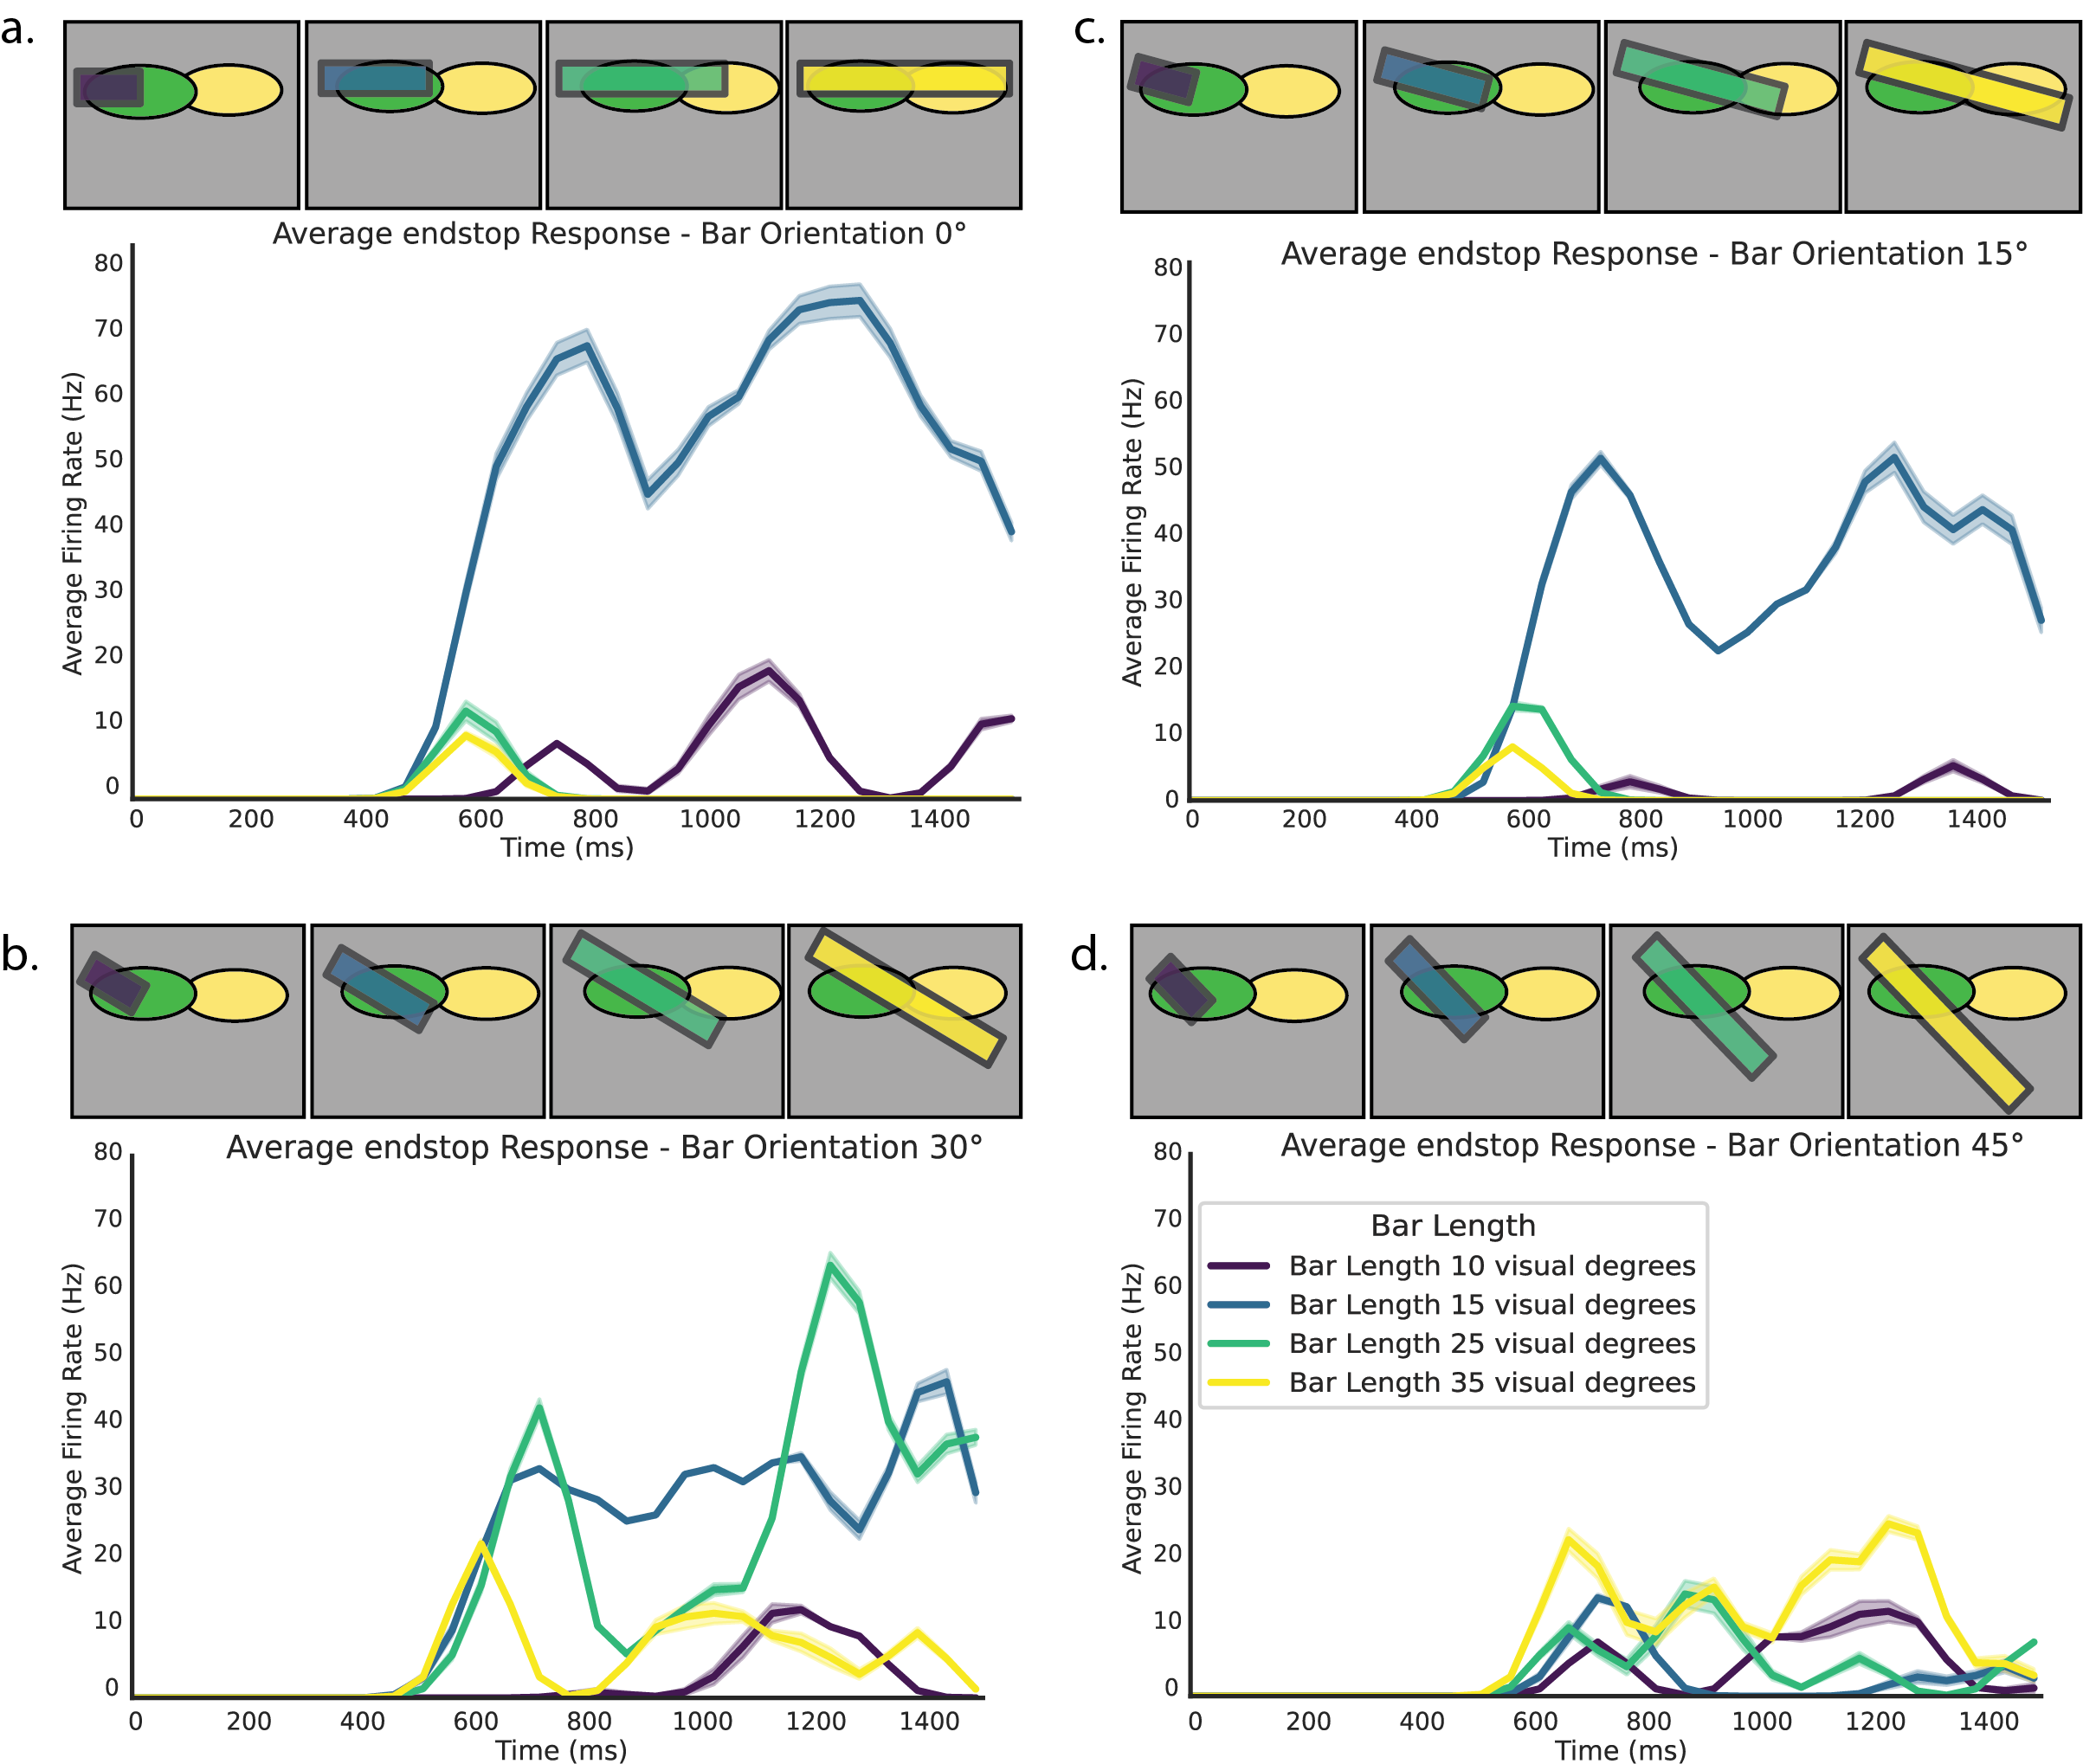
\includegraphics[width=1 \textwidth]{./figures/LIF_endstopping_length_orientation.png}
    \caption{Responses of the endstopped complex cells to different line segment lengths. The x-axis represents the length of the line segment in visual degrees, and the y-axis represents the firing rate of the complex cell in spikes per second (Hz). The cell types are colour coded of which the legend is located in d. The endstopped cell has an orientation preference of 0 degrees rotation, which is presented in figure a. The relative difference between bar lengths is greatest in this figure. Other figures show that with a greater orientation, peak firing rates decrease and that relative firing rate difference between bar lengths also decreases with more rotation.}
    \label{fig:endstopping}
\end{figure}


To gain a better understanding of the neural dynamics within the circuit, we also stimulated the model with a continuously growing bar. This approach allows us to visualize subtle differences related to the length of the bar at the population's preferred orientation, as shown in figure \ref{fig:endstopping_length}. This figure illustrates the elicited response of endstopped neurons to a bar that starts at the beginning of the receptive field and extends progressively into the endstopping field. The plot on the left shows the average firing rate (in Hz) of the neurons as a function of bar length (in visual degrees). The shaded area represents the variability around the mean firing rate. As depicted, the average firing rate increases steadily as the bar lengthens from 0 to approximately 15 visual degrees, peaking around 70 Hz. This peak indicates the optimal bar length that maximally activates the endstopped neurons within the receptive field. Beyond this length, the firing rate starts to decline, reflecting the inhibitory effect as the bar extends into the adjacent complex cell's receptive field.

The insets on the right side of the figure provide a visual representation of the bar's interaction with the receptive fields at different stages of its growth. The top inset shows the bar initially positioned within the receptive field of the endstopped neuron, eliciting a strong response. The middle inset illustrates the bar extending into the inhibitory zone, where the inhibitory feedback begins to reduce the firing rate. Finally, the bottom inset depicts the bar fully extending into the adjacent complex cell's receptive field, resulting in a significant reduction in the firing rate due to maximal inhibition. This figure effectively captures the dynamic response of endstopped neurons to varying bar lengths, highlighting the intricate balance between excitation and inhibition within the microcircuit. It reinforces the notion that recurrent inhibition plays a crucial role in modulating the activity of endstopped neurons, particularly in response to stimuli that extend beyond their classical receptive fields.

  \begin{figure}[H]
    \centering
    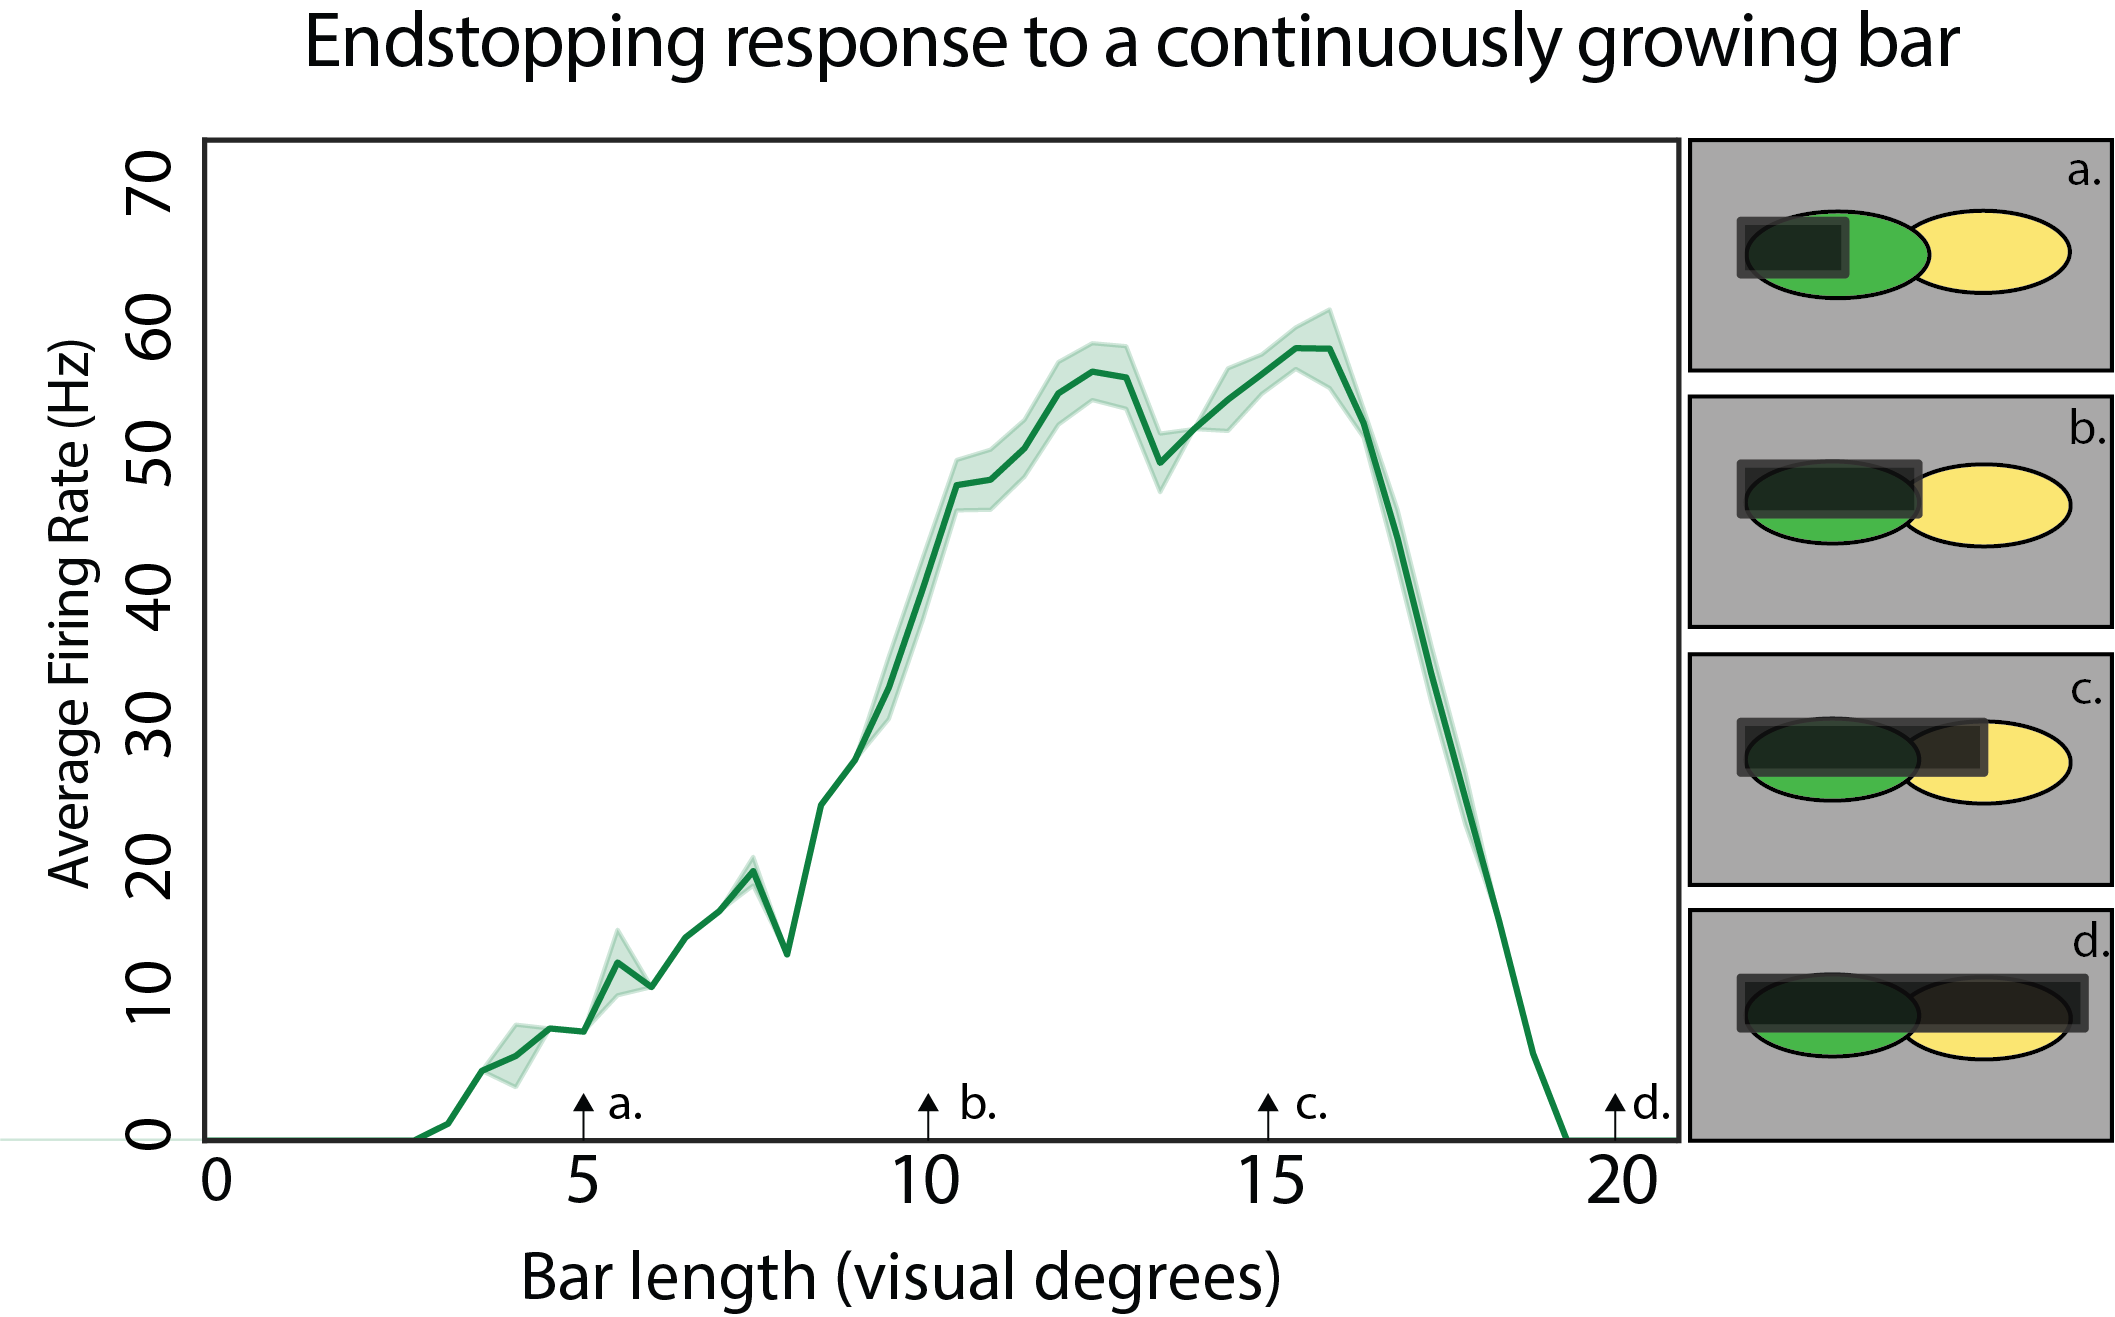
\includegraphics[width=1.0 \textwidth]{adjusted_figures/endstop_line_length.png}
    \caption{The response of an endstopping population stimulated with a continuously growing bar. Firing rates increase until the stimulus bar exceeds 15 visual degrees, after which firing is quickly dampened for longer inputs.}
    \label{fig:endstopping_length}
  \end{figure}

\subsection{Population activity illusory contours}
The figure presented showcases the responses of different cell types to visual stimuli designed to induce the perception of illusory contours. The left panels of each subfigure (a, b, and c) display the mean firing rates of various cell populations, including complex cells tuned to 90 degrees (\textit{mean complex}), complex cells tuned to 0 degrees (\textit{mean complex}), end-stop cells (\textit{mean endstop}), and pattern cells (\textit{mean pattern}). The right panels depict the spatial arrangement and the type of stimulus presented, which varies across the subfigures. Illusory contours are visual phenomena where contours are perceived without a corresponding gradient in the image's luminance or color. These are crucial for the perception of shapes and object boundaries in situations where actual physical boundaries are absent. The complex 90 cells, which are tuned to detect contours at 90-degree orientations, play a significant role in encoding these illusory contours.

In subfigure (a), the stimulus arrangement likely creates a strong illusion of contours aligned with the orientation preference of the complex 90 cells. This is evidenced by the robust mean firing rate of the \textit{mean complex 90 deg} cells, peaking at around 30 Hz, indicating a high level of activity in response to the perceived illusory contours. The elevated firing rates suggest that these cells are effectively encoding the illusion, signaling the presence of a boundary where none exists in the physical stimulus. When the stimulus is altered to disrupt the illusion, as seen in subfigures (b) and (c), the activity of the complex 90 cells changes significantly. In subfigure (b), the stimulus modification appears to partially disrupt the illusory contour. This is reflected in the reduced firing rate of the \textit{mean complex} cells compared to subfigure (a), though the response remains notable. This partial disruption suggests that the illusory contour is weakened but not entirely broken, resulting in a moderate decrease in the encoding efficiency of these cells.

In subfigure (c), the stimulus is further modified, presumably to completely break the illusion. The firing rate of the \textit{mean complex} cells drops significantly compared to subfigures (a) and (b). This substantial reduction in activity indicates that the complex 90 cells are no longer effectively encoding the illusory contour, as the stimulus no longer supports the perception of such a contour. The response of these cells now aligns more closely with their response to an actual absence of contours, highlighting their role in specifically detecting and encoding illusory boundaries. The right panels of each subfigure visually illustrate the stimulus configurations, showing how the spatial arrangement of elements impacts the perception of illusory contours. The color coding indicates the average firing rates, with warmer colors representing higher activity levels. The complex cells (dotted outlines) and end-stop cells (solid outlines) are shown in their spatial positions, providing a visual correlation between cell type location and stimulus-induced activity.

In summary, the complex 90 cells are crucial for encoding illusory contours, as evidenced by their high firing rates in response to stimuli that induce such perceptions. When the stimulus is altered to disrupt the illusion, the activity of these cells decreases accordingly. This suggests that the complex 90 cells are finely tuned to detect and encode the presence of contours, whether real or illusory, and their activity is a direct reflection of the strength of the perceived illusion. These findings underscore the importance of specific neural populations in the higher-order processing of visual information, particularly in the context of perceptual phenomena like illusory contours.

\begin{figure}[H]
  \centering
  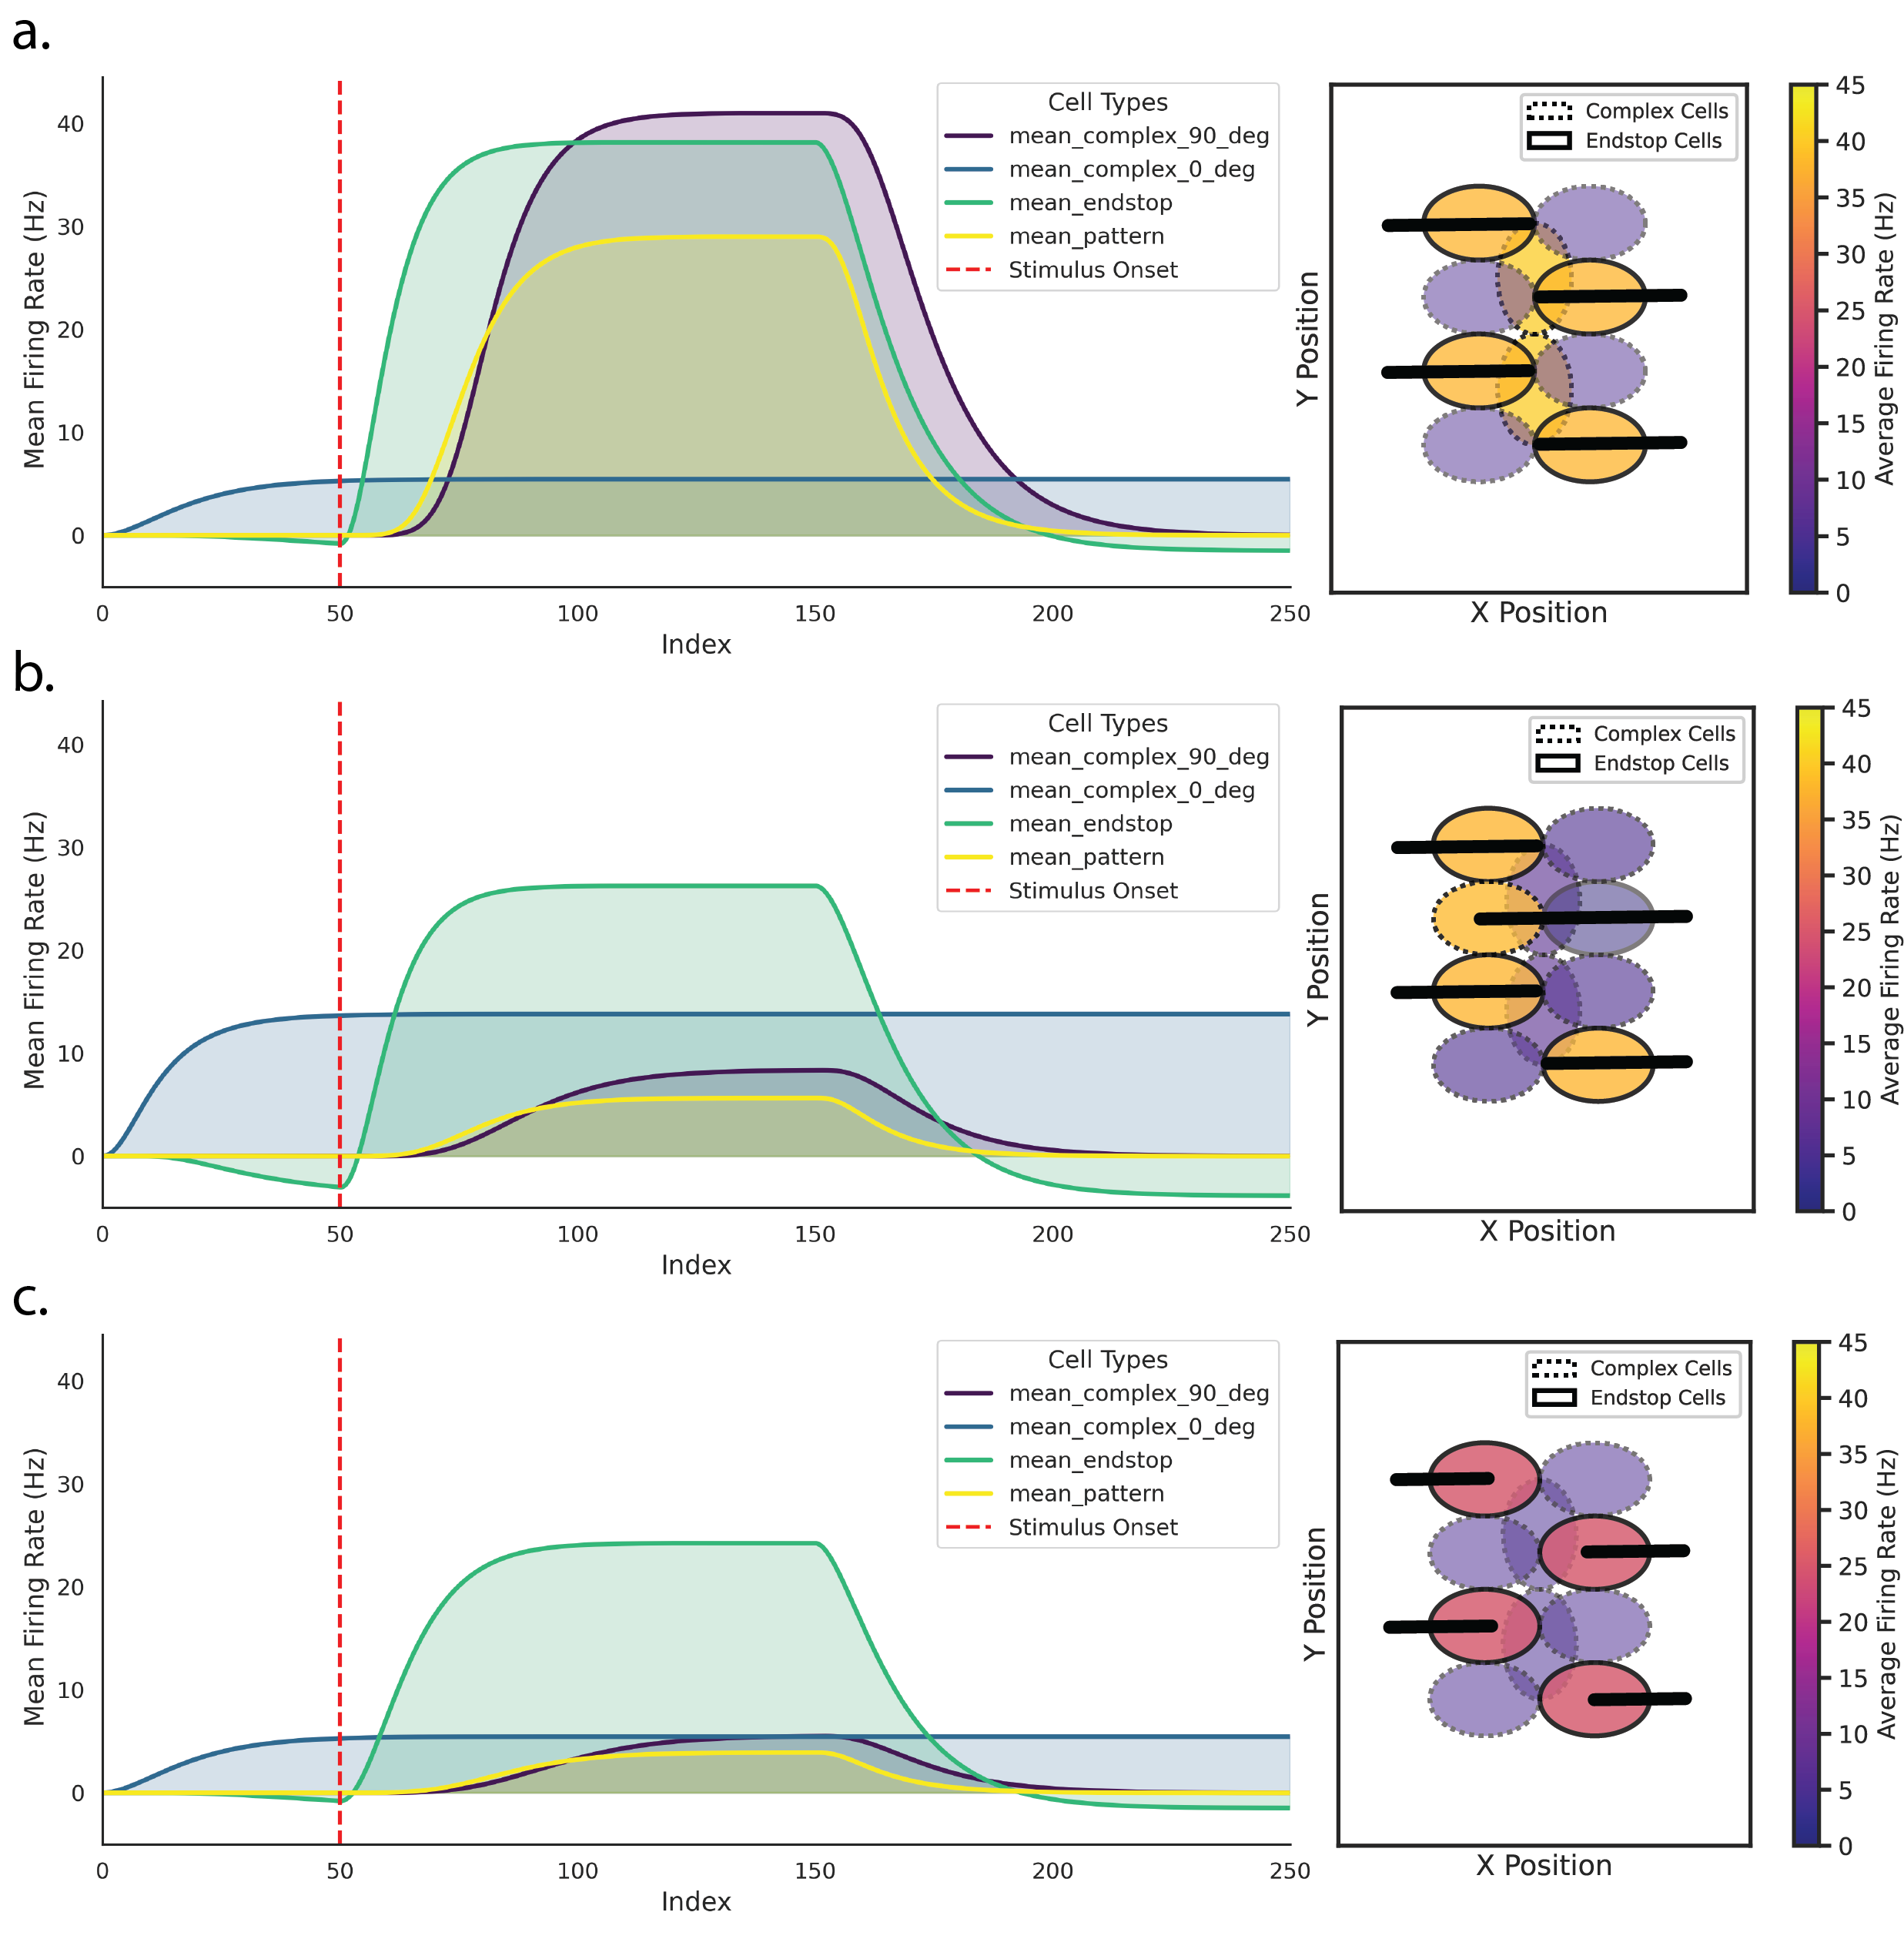
\includegraphics[width=1.0 \textwidth]{figures/Figure_Population_configs.png}
  \caption{a. The optimal input is given to the model, all inducers are the preferred orientation and are spatially aligned. All endstopped populations are very active and the complex endzones are not active, thus resulting in maximum representation of the illusory contour. b. In this example one of the inducers crosses the illusory contour, resulting in the abolishment of the illusion. The complex endzones increase in activity and thus is the endstopped cell decreased and no illusory contour is formed. c. Similarly, in this figure the inducer lines are not aligned enough the form a strong illusory contour. The complex endzones are not activated, but also the endstopped cells are not maximally stimulated. Therefore, the pattern cell is not stimulated enough and no illusory contour is formed.}
  \label{fig:population_contours}
\end{figure}

% \subsection{Representation real contours vs illusory contours in the model}


\newpage
\section{Discussion}
\setlength{\parindent}{12pt} The current model investigates the neural mechanisms underlying the representation of illusory contours within mouse V1, focusing on the role of endstopped cells to detect illusory inducing features and ultimately drive recurrent contour completion. We modelled endstopped cells with LIF point neurons, by creating a microcircuit that connect two adjacent populations of complex cells through inhibitory feedback connections that results in a decrease in firing whenever a stimulus edge is extended beyond the endstop receptive field. Our findings demonstrated that the endstopped caells are a critical step for the initial detections of illusory inducing local features and that they can be used to group retinotopically aligned line ends into a global illusory representation. To examine the global representation of the abutting grating a similar architecture that was used in the LIF model was implemented with mass neural population equations instead of the former LIF equations. Therefore, our two models had similar retinotopic architectures in which also the microcircuit structure that combined simple, complex, endstopped, and inhibitory cells was left intact, ensuring a stable firing rate for the recurrent amplification of illusory contour responses in the population model.
\setlength{\parindent}{0pt}
\bigbreak

\subsection{(LIF endstop) Recurrent inhibitory responsible for stable endstopping.} %no direct inhibition (check the original paper: silito 1977), why not? recurrent inhibition plays a role in balancing activation  \autocite{znamenskiyFunctionalSpecificityRecurrent2024}, \autocite{hanselMechanismOrientationSelectivity2012}
Results from the LIF model showed that recurrent inhibitory signals can be used to generate endstopping behaviour robust to stimuli variations of length and orientation. 

\subsection{Recurrent endstopping might explain second order features.} % simple cell \autocite{yazdanbakhshEndStoppingV12006}


\subsection{(Excitatory feature grouping) Endstopped Pattern and Complex cells create an excitatory recurrent network for boundary completion.} Also recurrent excitatory connection have been found in V1 \autocite{muirSpecificExcitatoryConnectivity2017}.

% Ji, Gamanut, Burkhalter, 2015. Modularity in the organisation of mouse V1; no clustering retinotopic equivalence but integrating distant
Additionally, the population mass neuron model predicts that complex cells, rather than  inhibitory V1 cells are the primary target of feedback signals that are responsible for the resulting illusory boundary completion. Additionally, population models demonstrated accurate responses to stimulus configurations that are close to eliciting an illusory response, however are varied, so they should not. Altogether, these findings indicate that recurrent activity induced by endstopping cells is essential for the robust segmentation of the abutting grating illusion. Additionally, population models showed that endstopped signals are sufficient to guide population activity to fill in details that are not present in the local feedforward input, but have behavioural relevance due to the collective meaning of the stimulus configuration, such as the representation of a visually occluded object.

\subsection{(Population) LM pattern cell grouping local features to build robust representation, driven by recurrent excitation of endstopped cells.}
% Ji, Gamanut, Burkhalter, 2015. Modularity in the organisation of mouse V1; no clustering retinotopic equivalence but integrating distant

\subsection{Broad feedback to orientation tuned complex cells have the ability to interpolate illusory contours}

\section{Limitations.}
\subsection{Deep learning strategies can help present many input, have the receptive fields be created through deep learning. To test hypothesis define the feedforward input architecture and find out what feedback structure the model comes up with when creating illusory contours. }

%---
%Idea is: no direct inhibition (check the original paper: silito 1977), why not? recurrent inhibition plays a role in balancing activation  \autocite{znamenskiyFunctionalSpecificityRecurrent2024}, \autocite{hanselMechanismOrientationSelectivity2012}

% If inhibition balances endstopping behaviour in the local circuit, why is integration of featuers excitatory? All endstopped cells are excitatory in nature (Endstopping V1 sensitive to contrast, excitatory subfield change to inhibitory, due to simple cell \autocite{yazdanbakhshEndStoppingV12006}), Also recurrent excitatory connection have been found in V1 \autocite{muirSpecificExcitatoryConnectivity2017}. 
%--
%Excitatory endstopped cells. Recurrent interactions to bind spatial features
The current model predicts that endstopped cells are excitatory cells that have complex responses as well as functional inhibitory endzones. Local excitatory recurrency has been demonstrated in other computational models to explain V1 responses to a overlapping plaid stimulus \autocite{muirSpecificExcitatoryConnectivity2017}. They found that a feedforward like to like scheme is not sufficient for the representation of a plaid stimulus. They examined how simple second-order relationships between neurons could sustain feature binding. 

\autocite{shinRecurrentPatternCompletion2023}.

% Balanced inhibitory activity
By systematically varying the stimulus length and orientation we observed that endstopping behaviour gradually decreased from when the ideal configuration was shown. We proposed that the main reason for the balanced endstopping is that the PV interneurons inhibit the simple cell population and do not project directly to the complex cell within the microcircuit. 

Studies such as those by Znamenskiy et al. (2024) and Hansel et al. (2012) highlight the importance of inhibitory feedback in stabilising feature-specific excitatory activity and supporting competition among neural ensembles. 


\begin{itemize}
  \item Endstopped cells are not directly inhibited by PV cells but recurrently in current model, why: Inhibitory feedback plays a crucial role in the balancing of feedforward input, not achievable in strictly feedforward networks. \autocite{znamenskiyFunctionalSpecificityRecurrent2024}, \autocite{hanselMechanismOrientationSelectivity2012} check recurrency inhibiton
  \item All endstopped cells are excitatory in nature (Endstopping V1 sensitive to contrast, excitatory subfield change to inhibitory, due to simple cell \autocite{yazdanbakhshEndStoppingV12006}), Also recurrent excitatory connection have been found in V1 \autocite{muirSpecificExcitatoryConnectivity2017}
\end{itemize}

\subsubsection{Population model predictions}
\begin{itemize}
  \item LM grouping local features to build global perceptions, integration of FF and FB in L2/3  % Ji, Gamanut, Burkhalter, 2015. Modularity in the organisation of mouse V1; no clustering retinotopic equivalence but integrating distant
  \item Recurrent input filling in informaton, population internal recurrency; increased firing during stable input
  \item ...
\end{itemize}

\subsection{Limitations.}
\begin{itemize}
  \item Deep learning optimisation
  \item Integrating illusory contours of curved inducers
  \item Real vs illusory contour representation, laminar dominance illusion (L2/3)
  \item ...
\end{itemize}
%---
%LIF model prediction
  %
  % Demonstrating how inhibitory feedback plays a crucial role in balancing feedforward input, which is not achievable in a strict feedforward network.

% Population model predictions
  % Population activity grouping into global percept, Feedforward and feedback integration in L2/3 visual cortex
    % Ji, Gamanut, Burkhalter, 2015. Modularity in the organisation of mouse V1; no clustering retinotopic equivalence but integrating distant
    % Bastos Predictive coding canonical column.

  % Recurrent input can fill in information (Population internal recurrency)
    % The feedback from pattern cells makes it possible to integrate multiple weak inputs to a strong output because of internal recurrency

% Lastly, the prediction that IC encoders are complex cells rather than inhibitory cells is supported by models of visual processing. Grossberg (1998) proposed that complex cells play a pivotal role in encoding illusory contours, integrating local edge information into a global perceptual framework. Fan et al. (2023) further demonstrated that deep neural networks incorporating recurrent connections could better represent illusory contours, suggesting that complex cells, with their ability to integrate and process recurrent signals, are the primary encoders of these visual phenomena. This distinction is crucial for understanding the neural mechanisms underlying illusory contour perception, as it highlights the role of complex cells in integrating local and global visual information through recurrent processing.
%----

% \subsection{Limitations}
% \subsubsection{Deep learning optimisation}
% The current model was tuned by hand to achieve the desired endstopping behaviour, combining multiple hierarchical levels of neuronal complexity. In future work, deep learning optimization techniques could be employed to automatically tune the model parameters and connectivity weights to achieve the desired endstopping behaviour. This would allow for a more systematic exploration of the parameter space and potentially uncover novel configurations that enhance the model's performance. Additionally, the use of deep learning optimization could help identify the most critical parameters and connections that contribute to endstopping, providing valuable insights into the underlying neural mechanisms. 

% This would make it possible to formulate a model consisting only of LIF cells in contrast to the mass neural models used in the current model. Additionally, the use of deep learning optimisation would make it possible to simulate the model on a larger scale, but also to simulate network responses to more continuously altered input configuration, testing it's robustness better.

% \subsubsection{Recurrent activity target}
% In the current model feedback from LM targets endstopped cells and complex cells but it is possible to also have another feedback loop to the simple cells for better spatial resolution. 

%   \subsubsection{Real vs illusory contour representation}
%   Electrophysiological it seems that the L4 simple cells are dominated by feedforward input and thus should not directly be influenced by illusory contours, the current model is indeed setup so that from L2/3 the endstopped cells converge onto higher visual areas and which send feedback to deeper layers of the visual cortex. 
%   Electrophysiology, deeper layers more active or superficial layers? should be feedback, normally feedback from higher visual areas target deeper layers, but in the case of illusory contours, it seems that feedback from higher visual areas target superficial layers. (need to check this in the literature, done in mice: Wyatte, filling in process; Shin IC encoder where?, Pak et al. 2019, feedback from LM to V1 superficial layers)

%   Shins et al. 2023 found IC encoder neurons that do boundary completion locally through feedback. We do it through feedback population. with the use of deep learning we could set the LIF weights in order to train instead of direct population feedback. 

%   This recurrent activity locally can be used to interpolate curves
%   \subsubsection{Feedback allows for orientation interpolation for curved surfaces.}
% As seen in the results with current mass models it is possible to instruct orientation specific illusory contours, however in other electrophysiological studies it is clear that there are cases in which the illusory contour is curved. This is not possible with the current model, but it is possible to extend the model to include feedback from higher visual areas to V1 to allow for orientation interpolation. This would allow for the model to generate curved illusory contours, which would be a more accurate representation of the visual system. A possible neuronal mechanism that would result in curved illusory contour is a broad feedback response that integrates multiple orientations around the inducing orientation. In other words, the orientation selective feedforward input from the endstopped cells to the higher visual Pattern cells would be integrated and give feedback to closely matched cells instead of only the same orientation tuning as in the current model. Additionally, known feedback mechanisms to local inhibitory cells in L2/3 could also be included for a more rich feedback response that fills in between occluding visual features.

 




% Illusory contours are a product of excitatory propagation in the visual system. While endstopping in V1 can initially occur through feedforward signals, feedback mechanisms are crucial for activating inhibitory end zones. Ferster and Miller (2000) demonstrated that orientation selectivity and endstopping in V1 are influenced by both feedforward and feedback processes. Shushruth et al. (2012) expanded on this by showing that recurrent processing within and between visual areas refines these responses, ensuring that the visual system can accurately detect and represent illusory contours. This dual mechanism underscores the complexity of visual processing, where initial excitatory signals are fine-tuned by inhibitory feedback to achieve precise perceptual outcomes.

% ...


 

% \subsection{Model predictions; results in the literature.}
%   \subsubsection{Recurrent inhibitory activty balances activity needed for stable endstopping.}

%   - Endstopped cells are crucial for the representation of illusory contours, and their orientation tuning is modulated by feedback signals from higher visual areas.

%   - Illusory contours are a product of excitatory propagation: Endstopping in V1 can occur through feedforward signals, but feedback mechanisms are essential for activating inhibitory end zones.

%   - Recurrent activity is essential for robust image segmentation, allowing the integration of local and global visual features.
%   - Recurrent connectivity between lower and higher visual areas (HVAs) helps refine visual representations, particularly in cases where feedforward information is ambiguous or incomplete.

%   - prediction: IC encoders are complex cells and not inhibitory cells. 

% \subsection{Limitations}
% \subsubsection{Deep learning optimisation}
% The current model was tuned by hand to achieve the desired endstopping behaviour, combining multiple hierarchical levels of neuronal complexity. In future work, deep learning optimization techniques could be employed to automatically tune the model parameters and connectivity weights to achieve the desired endstopping behaviour. This would allow for a more systematic exploration of the parameter space and potentially uncover novel configurations that enhance the model's performance. Additionally, the use of deep learning optimization could help identify the most critical parameters and connections that contribute to endstopping, providing valuable insights into the underlying neural mechanisms. 

% This would make it possible to formulate a model consisting only of LIF cells in contrast to the mass neural models used in the current model. Additionally, the use of deep learning optimisation would make it possible to simulate the model on a larger scale, but also to simulate network responses to more continuously altered input configuration, testing it's robustness better.

% \subsubsection{Recurrent activity target}
% In the current model feedback from LM targets endstopped cells and complex cells but it is possible to also have another feedback loop to the simple cells for better spatial resolution. 

%   \subsubsection{Real vs illusory contour representation}
%   Electrophysiological it seems that the L4 simple cells are dominated by feedforward input and thus should not directly be influenced by illusory contours, the current model is indeed setup so that from L2/3 the endstopped cells converge onto higher visual areas and which send feedback to deeper layers of the visual cortex. 
%   Electrophysiology, deeper layers more active or superficial layers? should be feedback, normally feedback from higher visual areas target deeper layers, but in the case of illusory contours, it seems that feedback from higher visual areas target superficial layers. (need to check this in the literature, done in mice: Wyatte, filling in process; Shin IC encoder where?, Pak et al. 2019, feedback from LM to V1 superficial layers)

%   Shins et al. 2023 found IC encoder neurons that do boundary completion locally through feedback. We do it through feedback population. with the use of deep learning we could set the LIF weights in order to train instead of direct population feedback. 

%   This recurrent activity locally can be used to interpolate curves
%   \subsubsection{Feedback allows for orientation interpolation for curved surfaces.}
% As seen in the results with current mass models it is possible to instruct orientation specific illusory contours, however in other electrophysiological studies it is clear that there are cases in which the illusory contour is curved. This is not possible with the current model, but it is possible to extend the model to include feedback from higher visual areas to V1 to allow for orientation interpolation. This would allow for the model to generate curved illusory contours, which would be a more accurate representation of the visual system. A possible neuronal mechanism that would result in curved illusory contour is a broad feedback response that integrates multiple orientations around the inducing orientation. In other words, the orientation selective feedforward input from the endstopped cells to the higher visual Pattern cells would be integrated and give feedback to closely matched cells instead of only the same orientation tuning as in the current model. Additionally, known feedback mechanisms to local inhibitory cells in L2/3 could also be included for a more rich feedback response that fills in between occluding visual features.

% The feedback from pattern cells makes it possible to integrate multiple weak inputs to a strong output because of internal recurrency, 

\newpage
\printbibliography

\end{document}